\subsection{Simulazioni con algoritmo di Metropolis}

Le simulazioni considerate in questa sottosezione sono state effettuate con l'algoritmo di Metropolis, la cui 
implementazione è riportata in seguito. Per ogni mossa Monte-Carlo, viene tentato un numero di singole inversioni degli spin 
pari al numero di siti reticolari del modello stesso.

\begin{minted}[frame=lines, fontsize=\small, bgcolor=blue!10, breaklines = true]{nim}
  proc metropolisMove*(modIsing: var seq[seq[int]], rg: var PCG, temp: float32, acc: float32, nspin: int, accettate: var int) = 
  # Algoritmo di Metropolis per evolvere il modello di Ising 2D
  # Per ogni MC-move, provo a fare nspin * nspin inversioni degli spin
  # perchè nspin è "il lato" del reticolo quadrato considerato

  # Indice per selezionare lo spin
  var 
      nmove = int(nspin * nspin)
      diffE: float32
      xcoor, ycoor, appo: int
      up, down, left, right: int

  for i in 0..<nmove:

      # Seleziono casualmente uno spin facente parte del modello
      xcoor = int(floor(rg.rand(float32(0), float32(nspin)))) mod nspin
      ycoor = int(floor(rg.rand(float32(0), float32(nspin)))) mod nspin

      # Determino quali sono i primi vicini in questo caso (facendo attenzione a bc)
      down = (ycoor + 1) mod nspin
      right = (xcoor + 1) mod nspin
      up = (ycoor - 1 + nspin) mod nspin
      left = (xcoor - 1 + nspin) mod nspin

      # Calcolo i contributi energetici
      appo = modIsing[xcoor][ycoor]
      diffE = 2 * acc * float32(appo) * float32((modIsing[right][ycoor] + modIsing[left][ycoor] + modIsing[xcoor][up] + modIsing[xcoor][down]))

      if diffE < 0:
          modIsing[xcoor][ycoor] = -appo
          accettate += 1

      elif rg.rand() < exp(-diffE/temp):
          modIsing[xcoor][ycoor] = -appo
          accettate += 1
\end{minted}   



\subsubsection{Termalizzazione}

Il sistema viene inizializzato con tutti gli spin orientati up (ossia con valore pari ad 1), poichè questo consente di avere delle 
termalizzazioni di durata inferiore. Come è possibile osservare nelle figure riportate in seguito, la fase di transitorio è praticamente 
istantanea per temperature minori della temperatura critica o nettamente superiori. Nell'intorno di $T_c$ si osservano termalizzazioni 
più lunghe, che risultano essere di circa 500 mosse Monte-Carlo per $T\,=\,2.5$. Sebbene l'algoritmo di Metropolis non sia adeguato 
per caratterizzare il punto critico, potrebbe essere comunque interessante valutare cosa accada per $T\,\in\,\left\{2.1,\,2.2,\,2.3,\,2.4\right\}$, 
perchè il confronto con i risultati prodotti con l'algoritmo di Wolff sarebbe comunque significativo. Per questo motivo, oltre allo 
studio della termalizzazione sul range di temperature "ampio" riportato in precedenza, ho effettuato uno studio più focalizzato sull'
intorno del punto critico, osservando come per $T\,\to\,T_c^+$ la durata della fase di transitorio risulti essere nettamente maggiore, 
richiedendo oltre 10000 mosse Monte-Carlo. Inoltre, nell'intorno del punto critico, le fluttuazioni nella magnetizzazione, parametro 
d'ordine per il modello di Ising, persistono per un numero considerevole di mosse MC, il che implica con ogni probabilità che saranno 
necessari dei blocchi di dimensioni maggiori nell'intorno del punto critico. Le simulazioni successive sono state svolte con 500 mosse 
Monte-Carlo di termalizzazione, tranne quelle nell'intorno di $T_c$ le quali hanno richiesto una termalizzaione di 10000 mosse MC.


\vspace*{\fill}

\begin{figure}[htbp]
    \centering
    \begin{minipage}{0.45\textwidth}  
      \centering
      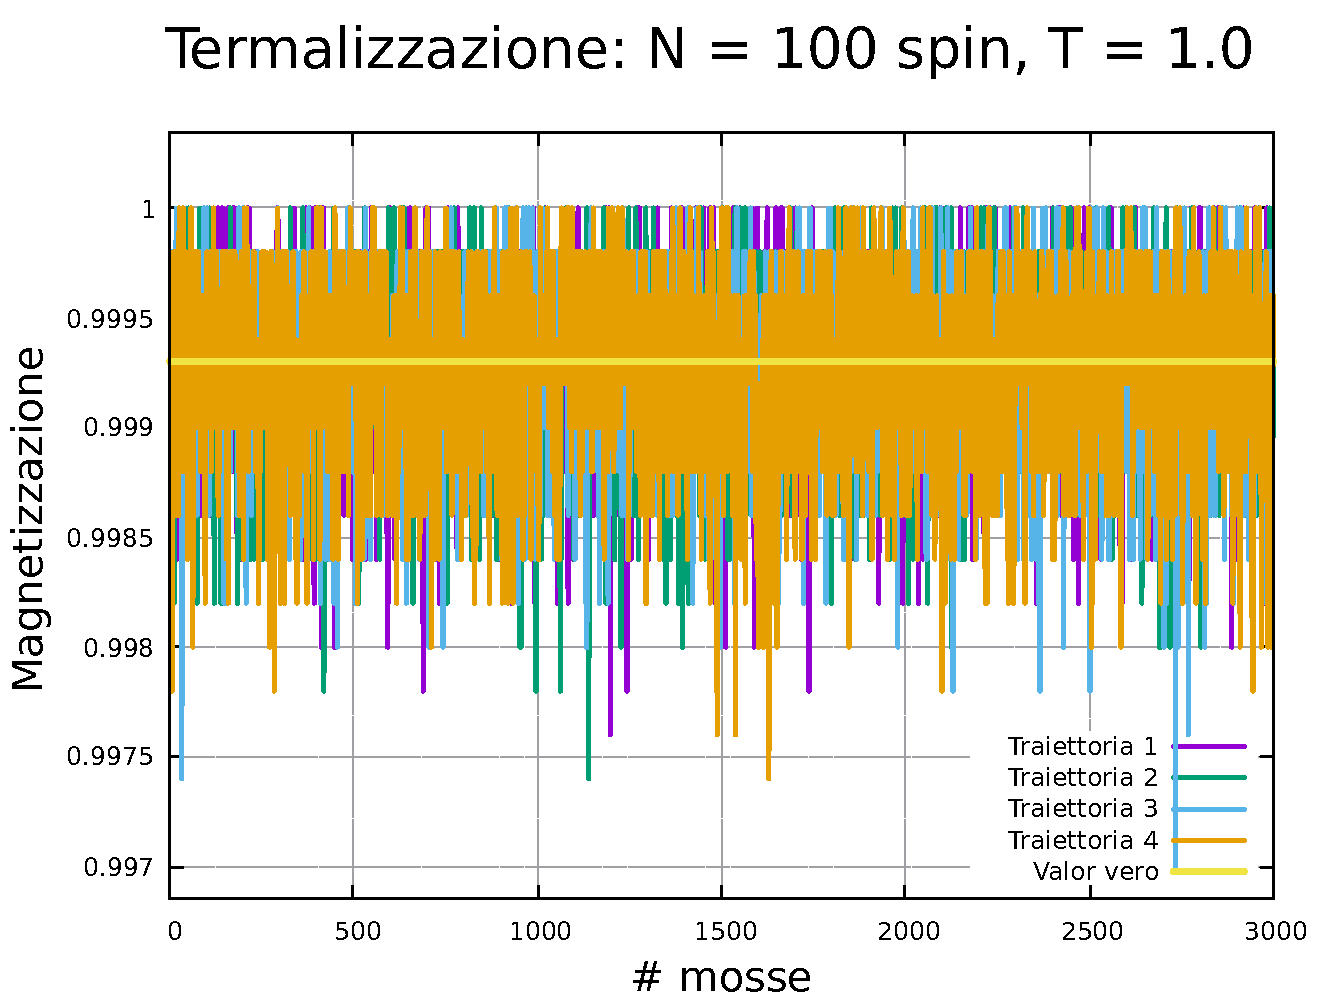
\includegraphics[page=1, width=\textwidth]{Immagini/simIsing2D/metro/term/term_100_1.0.pdf}
      \caption{$T\,=\,1.0$}
    \end{minipage}\hfill
    \begin{minipage}{0.45\textwidth}  
      \centering
      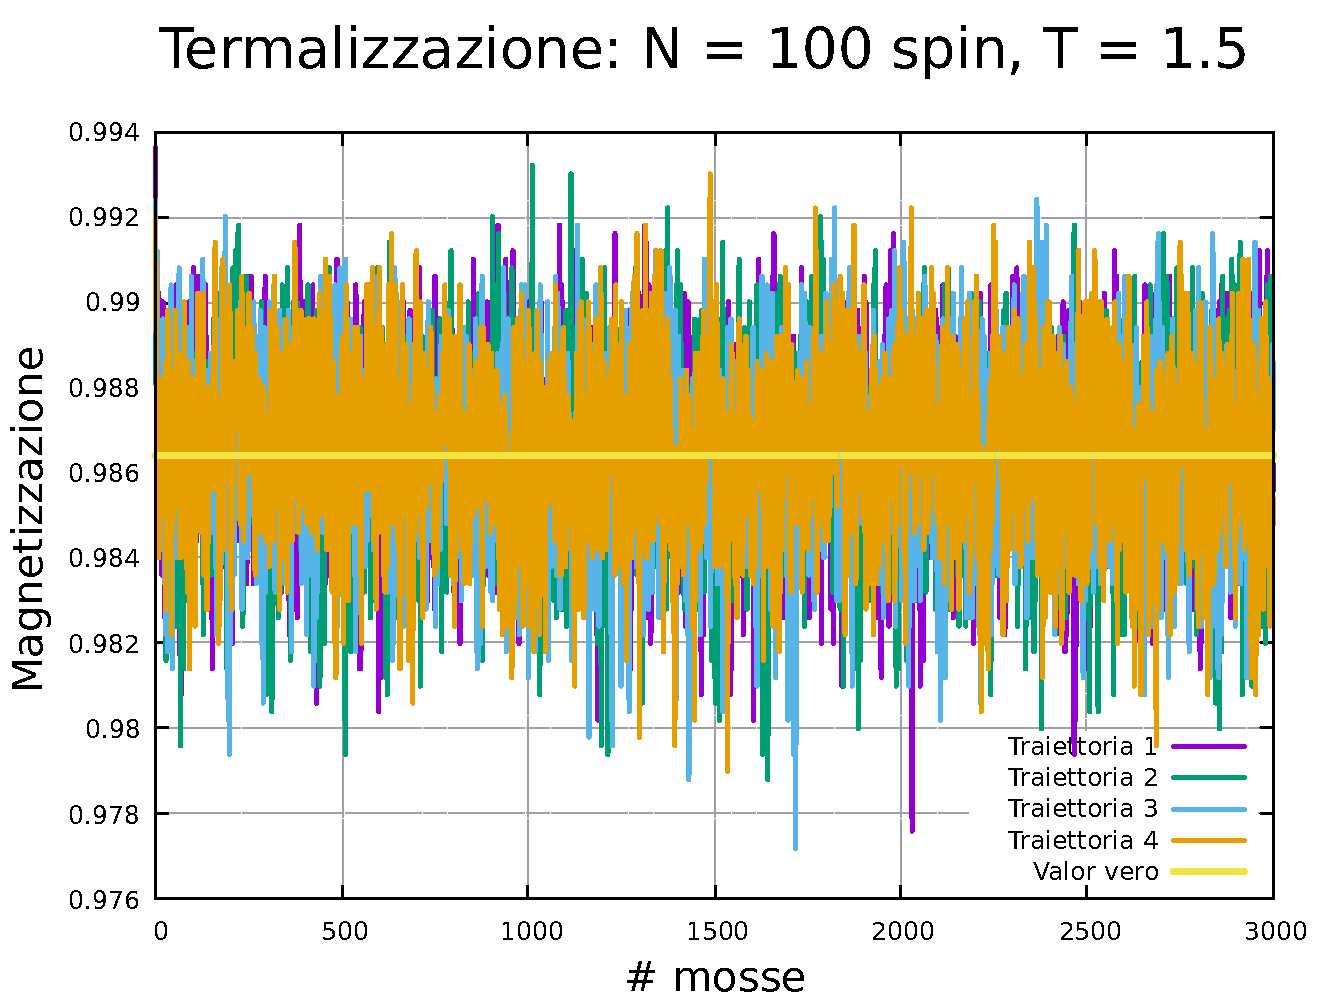
\includegraphics[page=1, width=\textwidth]{Immagini/simIsing2D/metro/term/term_100_1.5.pdf}
      \caption{$T\,=\,1.5$}
    \end{minipage}
    \vskip\baselineskip 

    \begin{minipage}{0.45\textwidth}  
        \centering
        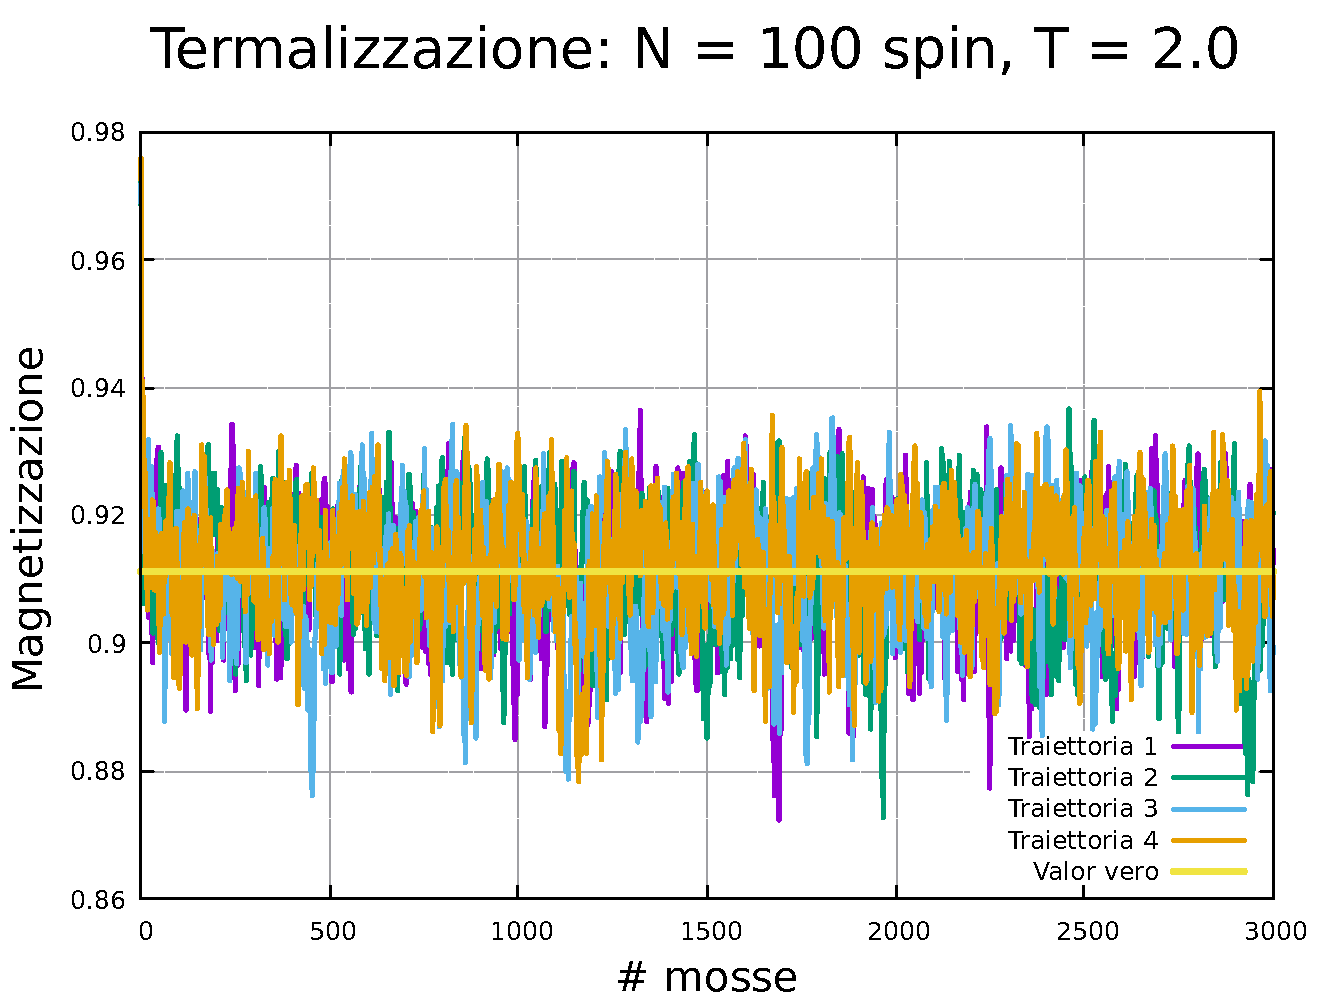
\includegraphics[page=1, width=\textwidth]{Immagini/simIsing2D/metro/term/term_100_2.0.pdf}
        \caption{$T\,=\,2.0$}
      \end{minipage}\hfill
      \begin{minipage}{0.45\textwidth}  
        \centering
        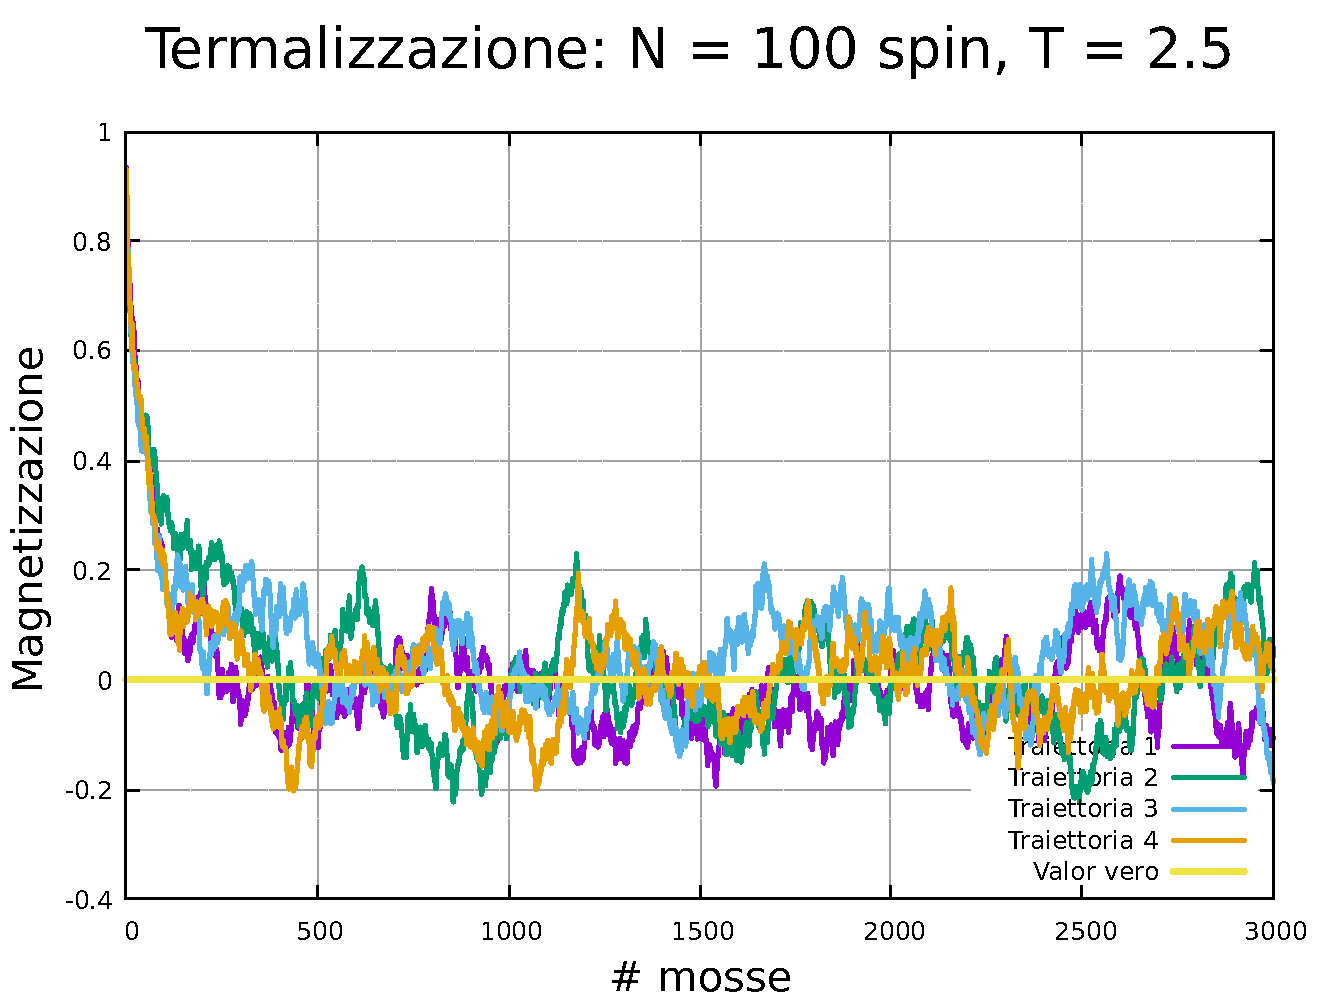
\includegraphics[page=1, width=\textwidth]{Immagini/simIsing2D/metro/term/term_100_2.5.pdf}
        \caption{$T\,=\,2.5$}
      \end{minipage}
    \vskip\baselineskip 
  
    \begin{minipage}{0.45\textwidth}  
      \centering
      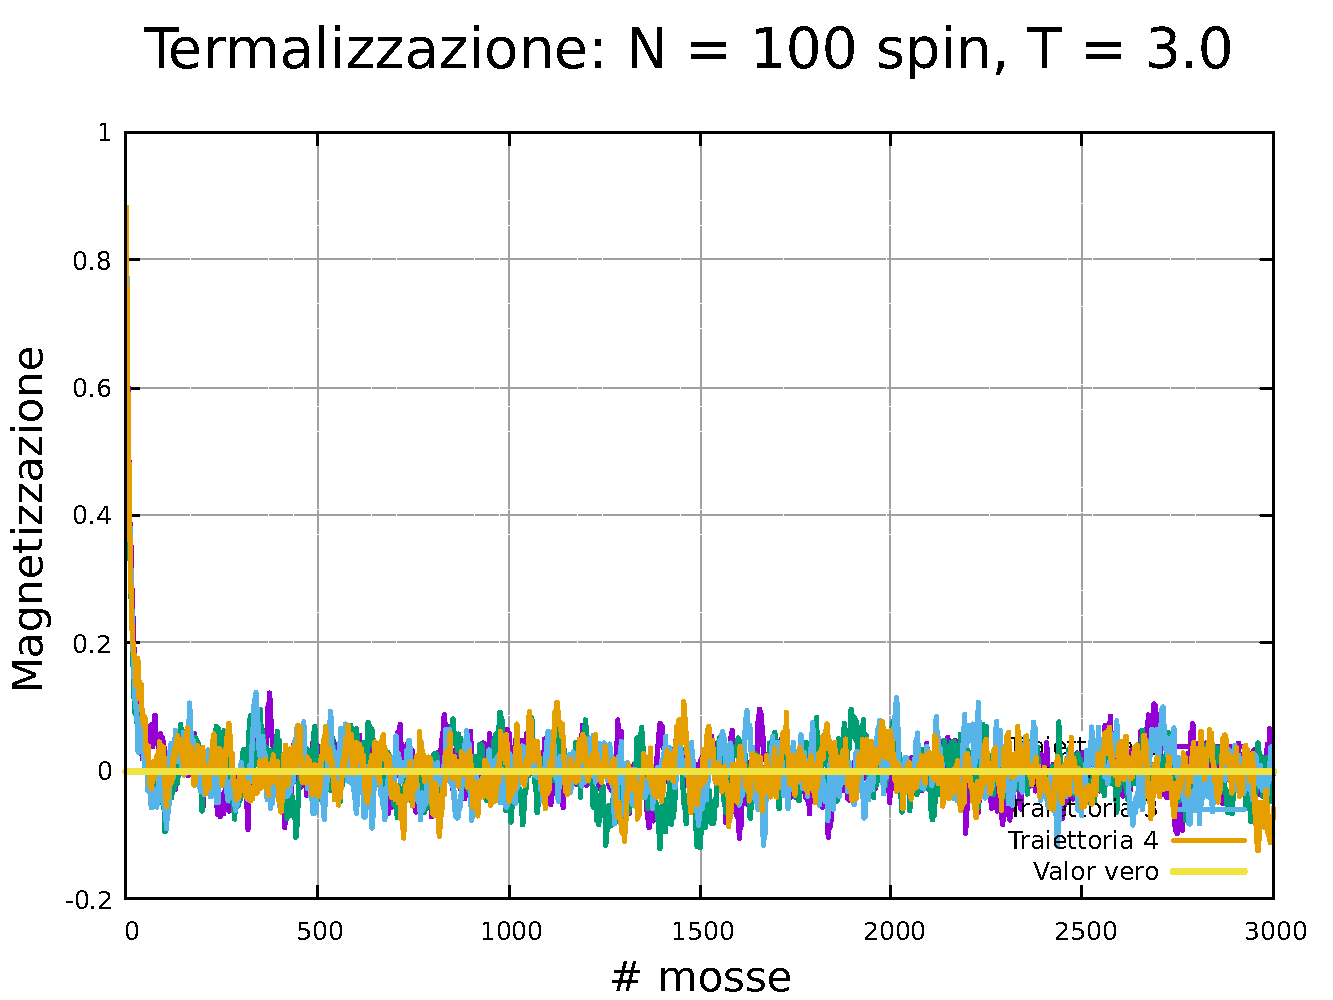
\includegraphics[page=1, width=\textwidth]{Immagini/simIsing2D/metro/term/term_100_3.0.pdf}
      \caption{$T\,=\,3.0$}
    \end{minipage}\hfill
    \begin{minipage}{0.45\textwidth}  
      \centering
      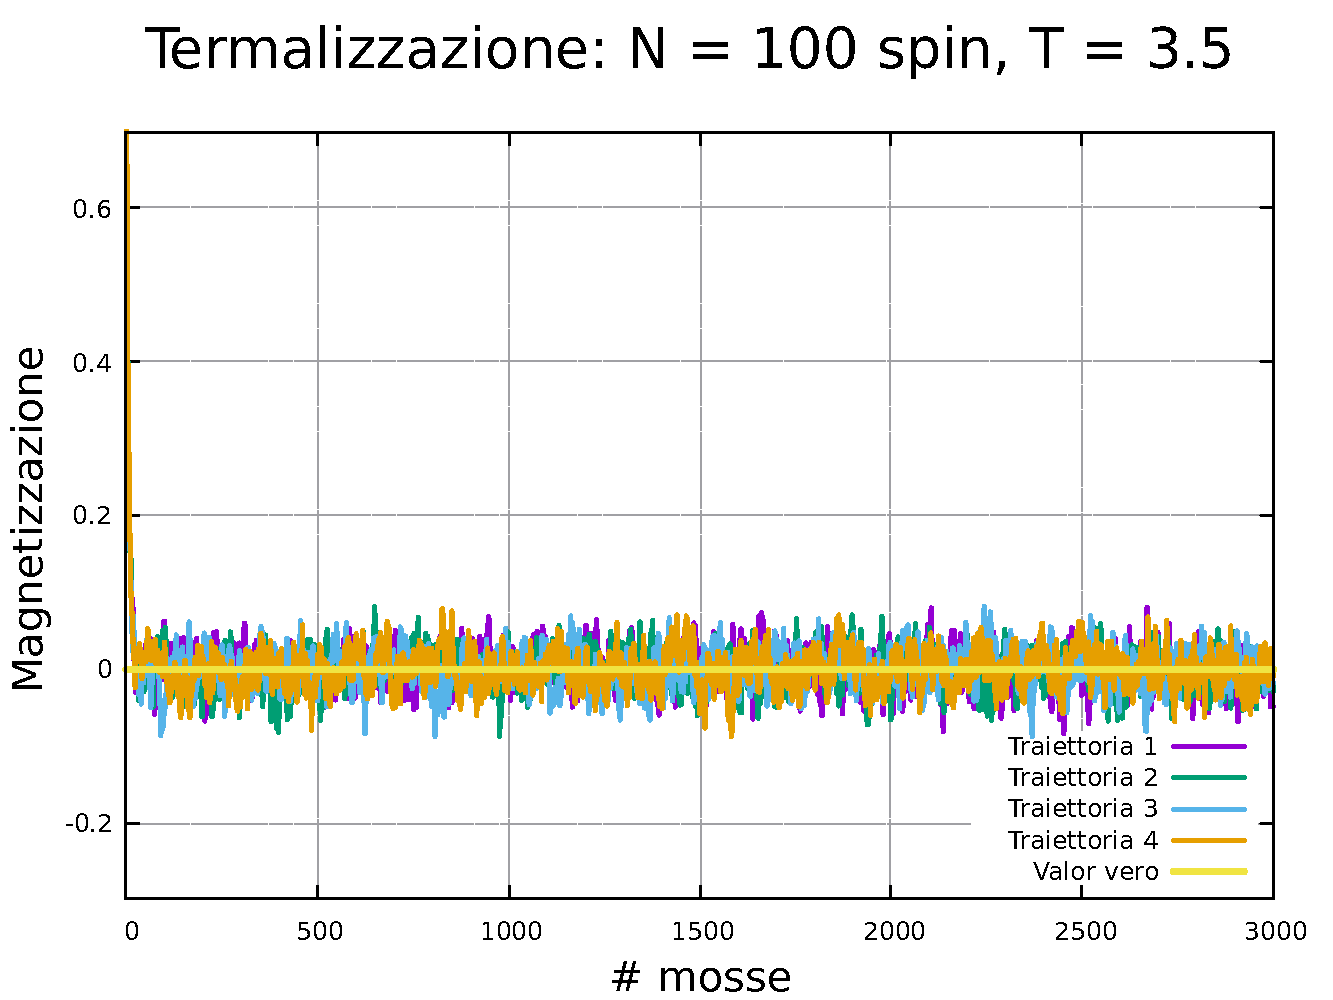
\includegraphics[page=1, width=\textwidth]{Immagini/simIsing2D/metro/term/term_100_3.5.pdf}
      \caption{$T\,=\,3.5$}
    \end{minipage}
    \caption{Studio della termalizzazione di un modello di Ising 2D costituito da $100 \times 100$ spin.}
\end{figure}

\vspace*{\fill}



\vspace*{\fill}

\begin{figure}[htbp]
    \centering
    \begin{minipage}{0.45\textwidth}  
      \centering
      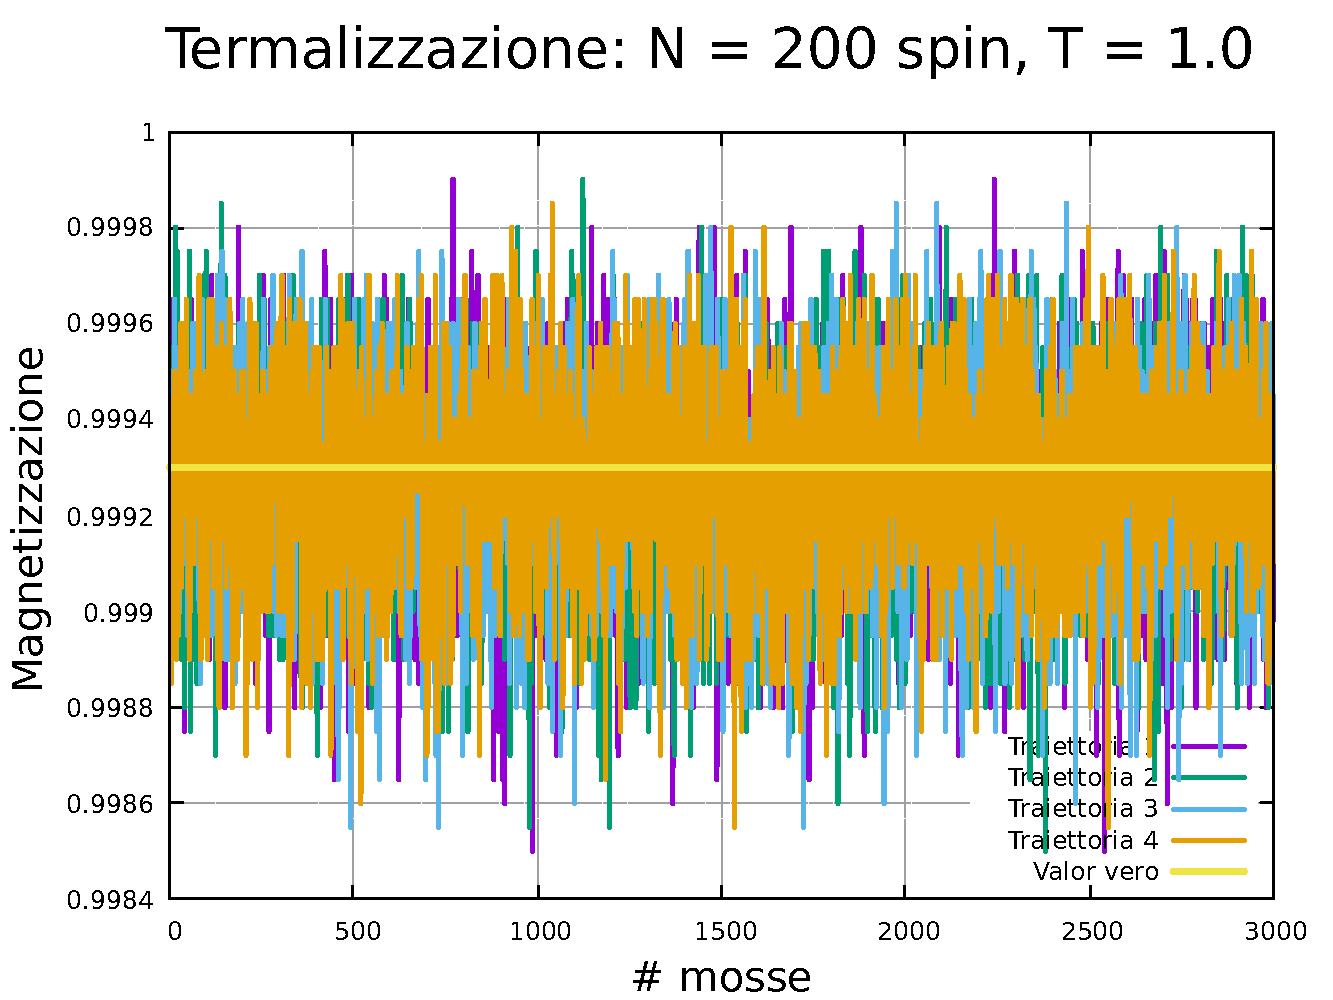
\includegraphics[page=1, width=\textwidth]{Immagini/simIsing2D/metro/term/term_200_1.0.pdf}
      \caption{$T\,=\,1.0$}
    \end{minipage}\hfill
    \begin{minipage}{0.45\textwidth}  
      \centering
      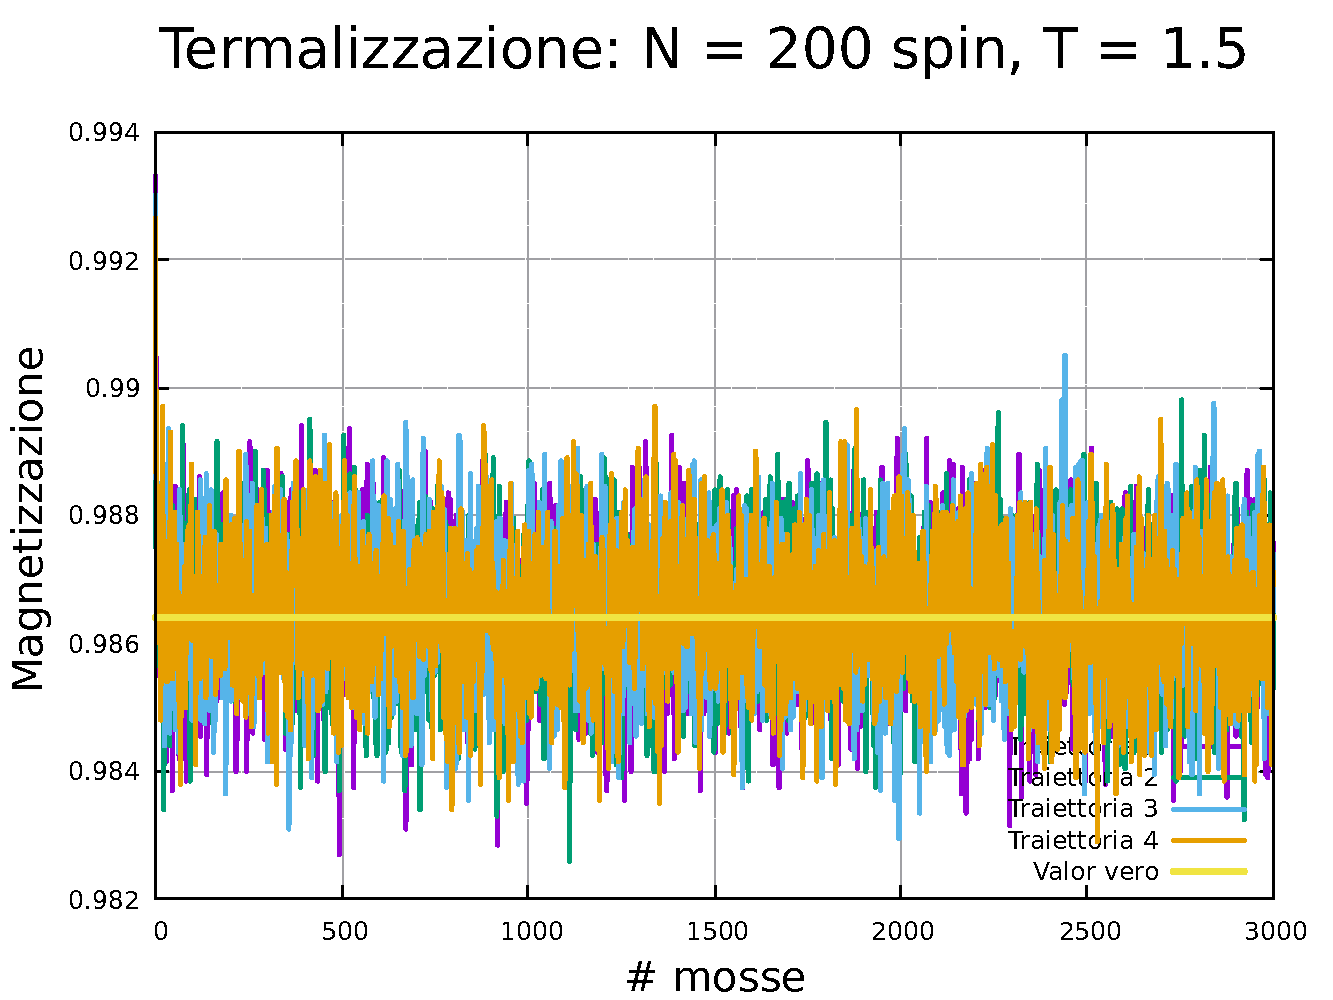
\includegraphics[page=1, width=\textwidth]{Immagini/simIsing2D/metro/term/term_200_1.5.pdf}
      \caption{$T\,=\,1.5$}
    \end{minipage}
    \vskip\baselineskip 
  
    \begin{minipage}{0.45\textwidth}  
      \centering
      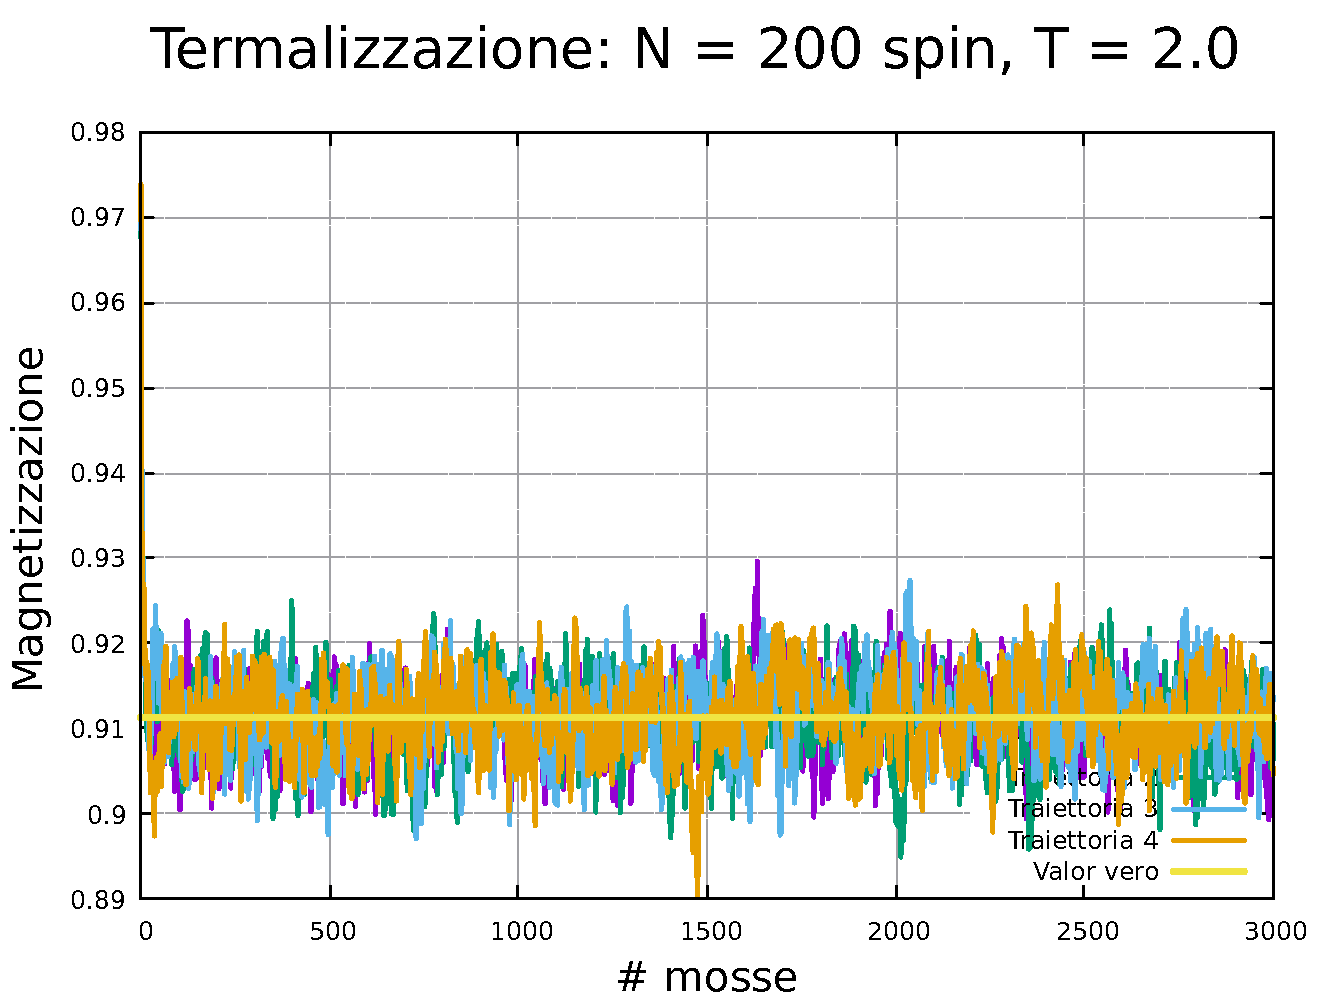
\includegraphics[page=1, width=\textwidth]{Immagini/simIsing2D/metro/term/term_200_2.0.pdf}
      \caption{$T\,=\,2.0$}
    \end{minipage}\hfill
    \begin{minipage}{0.45\textwidth}  
      \centering
      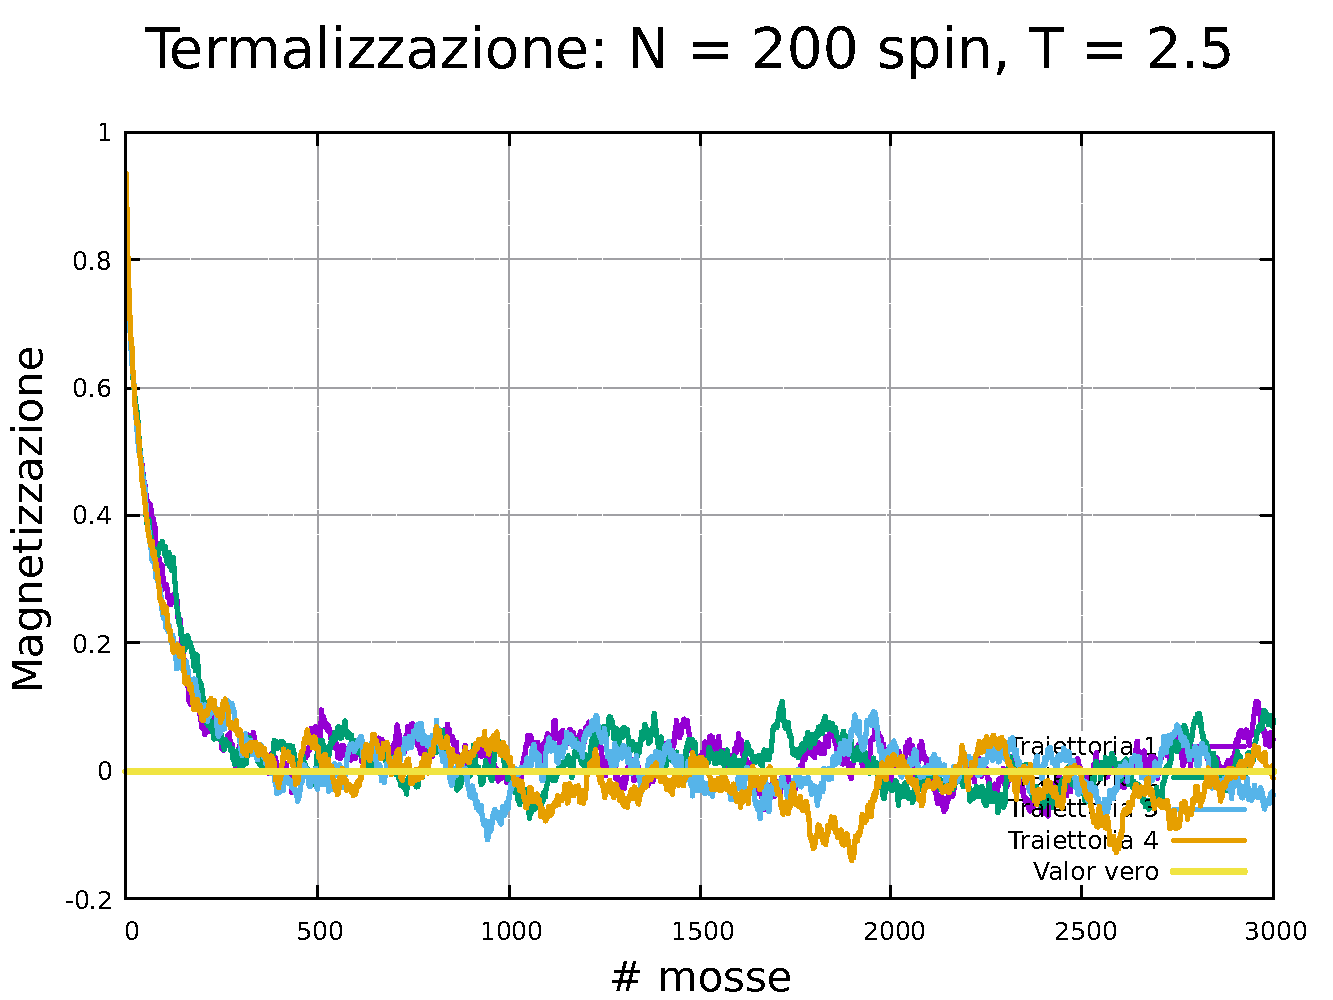
\includegraphics[page=1, width=\textwidth]{Immagini/simIsing2D/metro/term/term_200_2.5.pdf}
      \caption{$T\,=\,2.5$}
    \end{minipage}
    \vskip\baselineskip 

    \begin{minipage}{0.45\textwidth}  
        \centering
        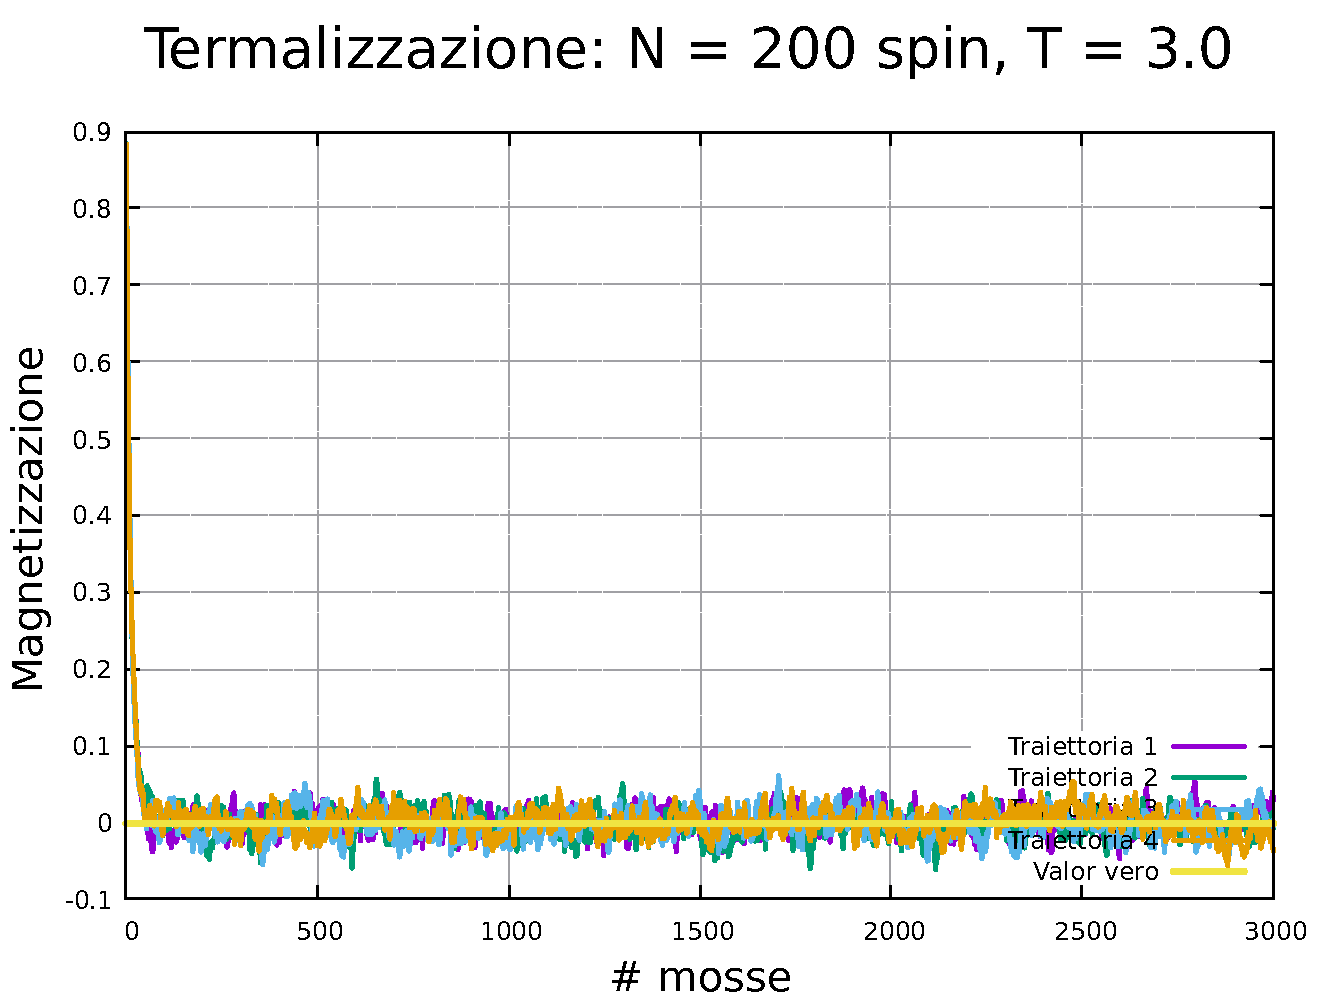
\includegraphics[page=1, width=\textwidth]{Immagini/simIsing2D/metro/term/term_200_3.0.pdf}
        \caption{$T\,=\,3.0$}
      \end{minipage}\hfill
      \begin{minipage}{0.45\textwidth}  
        \centering
        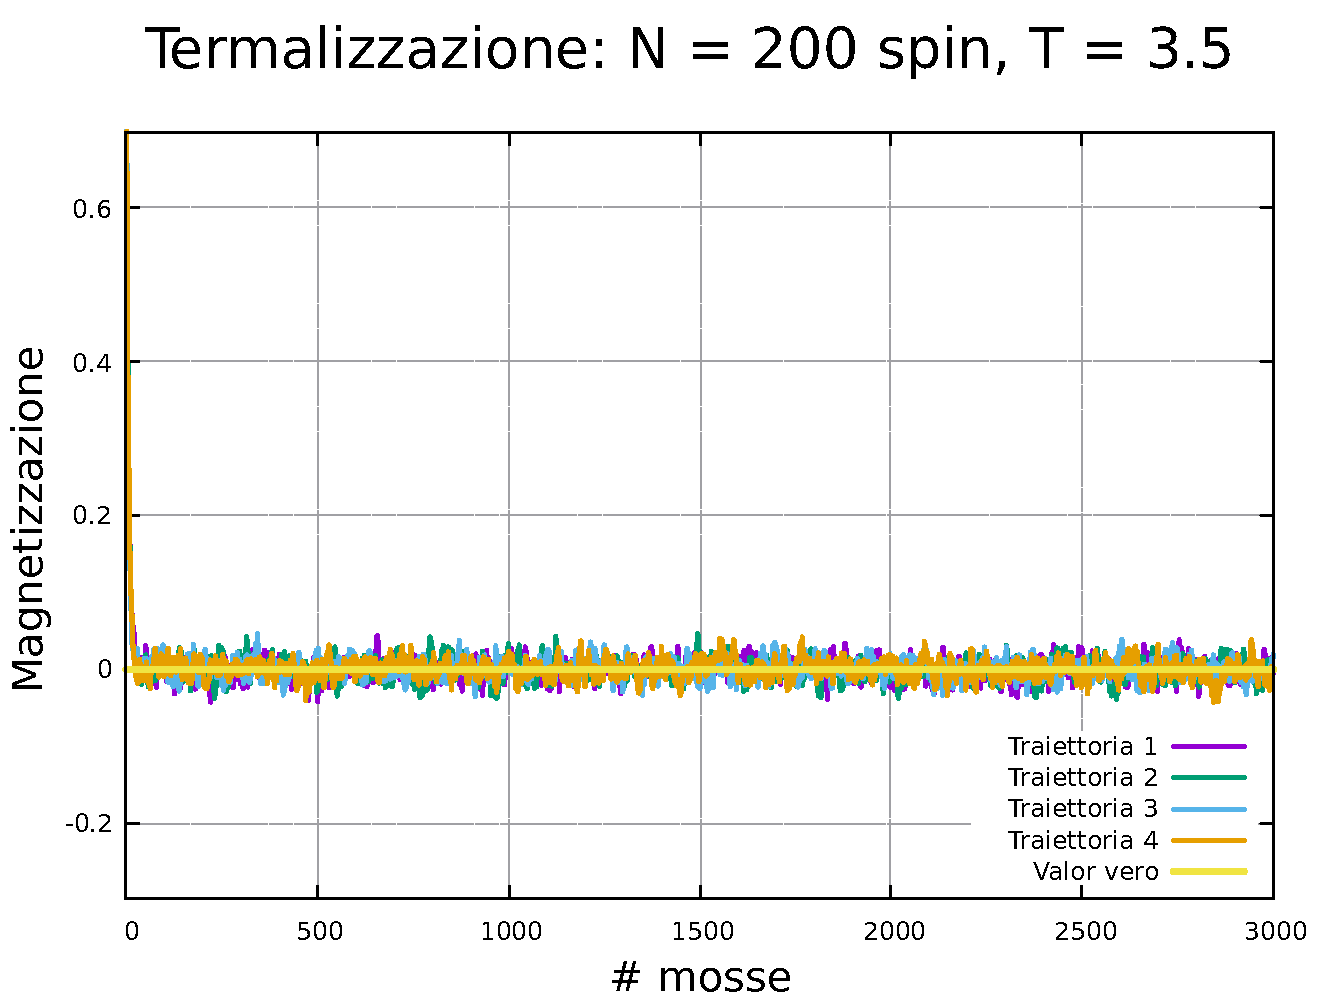
\includegraphics[page=1, width=\textwidth]{Immagini/simIsing2D/metro/term/term_200_3.5.pdf}
        \caption{$T\,=\,3.5$}
    \end{minipage}

    \caption{Studio della termalizzazione di un modello di Ising 2D costituito da $200 \times 200$ spin.}
\end{figure}

\vspace*{\fill}



\vspace*{\fill}

\begin{figure}[htbp]
    \centering
    \begin{minipage}{0.45\textwidth}  
      \centering
      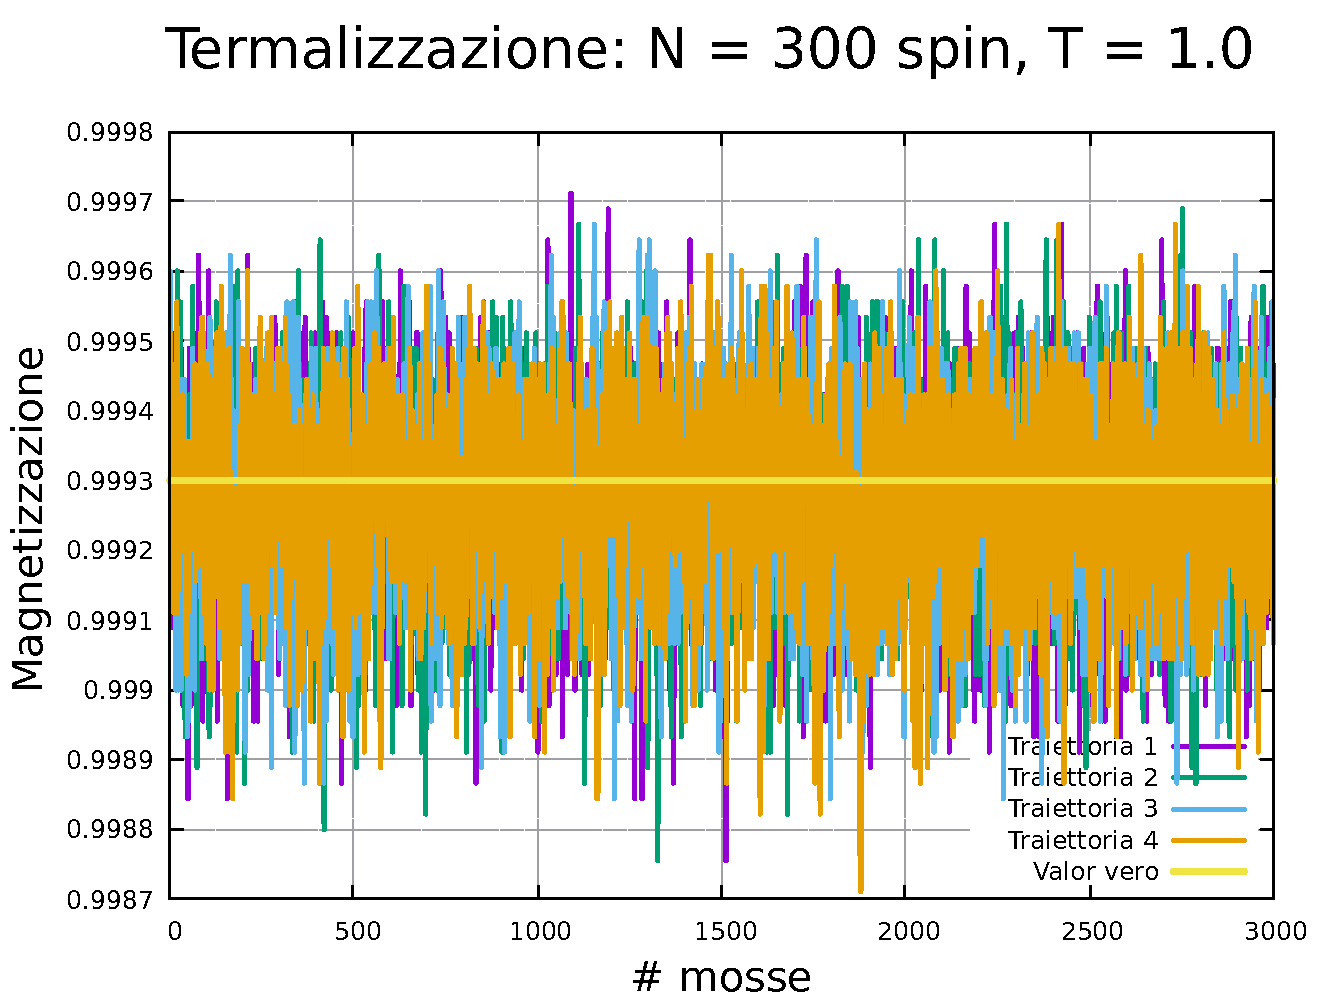
\includegraphics[page=1, width=\textwidth]{Immagini/simIsing2D/metro/term/term_300_1.0.pdf}
      \caption{$T\,=\,1.0$}
    \end{minipage}\hfill
    \begin{minipage}{0.45\textwidth}  
      \centering
      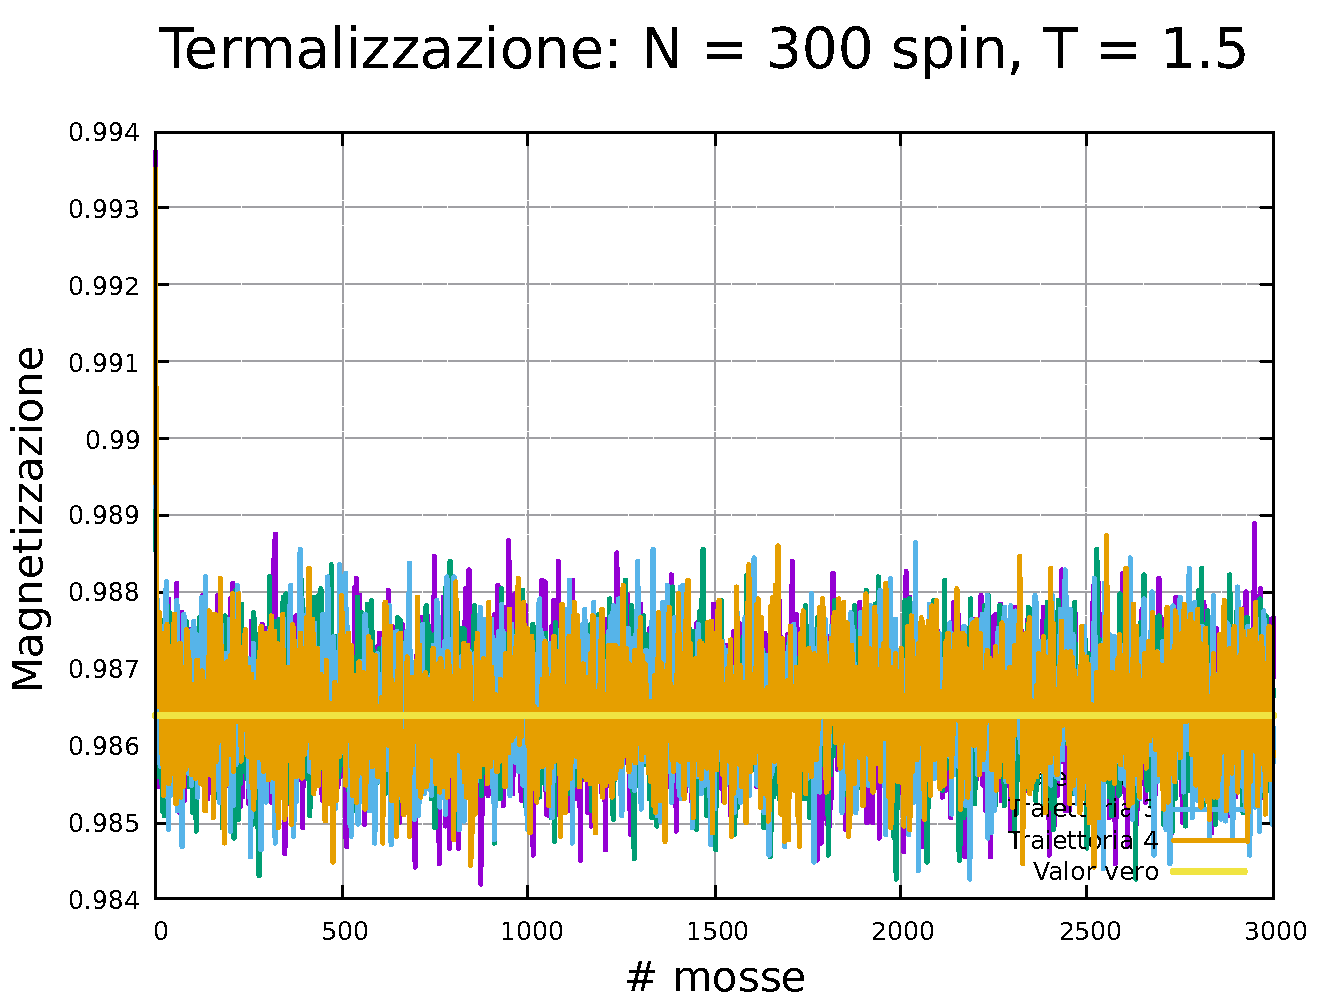
\includegraphics[page=1, width=\textwidth]{Immagini/simIsing2D/metro/term/term_300_1.5.pdf}
      \caption{$T\,=\,1.5$}
    \end{minipage}
    \vskip\baselineskip 

    \begin{minipage}{0.45\textwidth}  
        \centering
        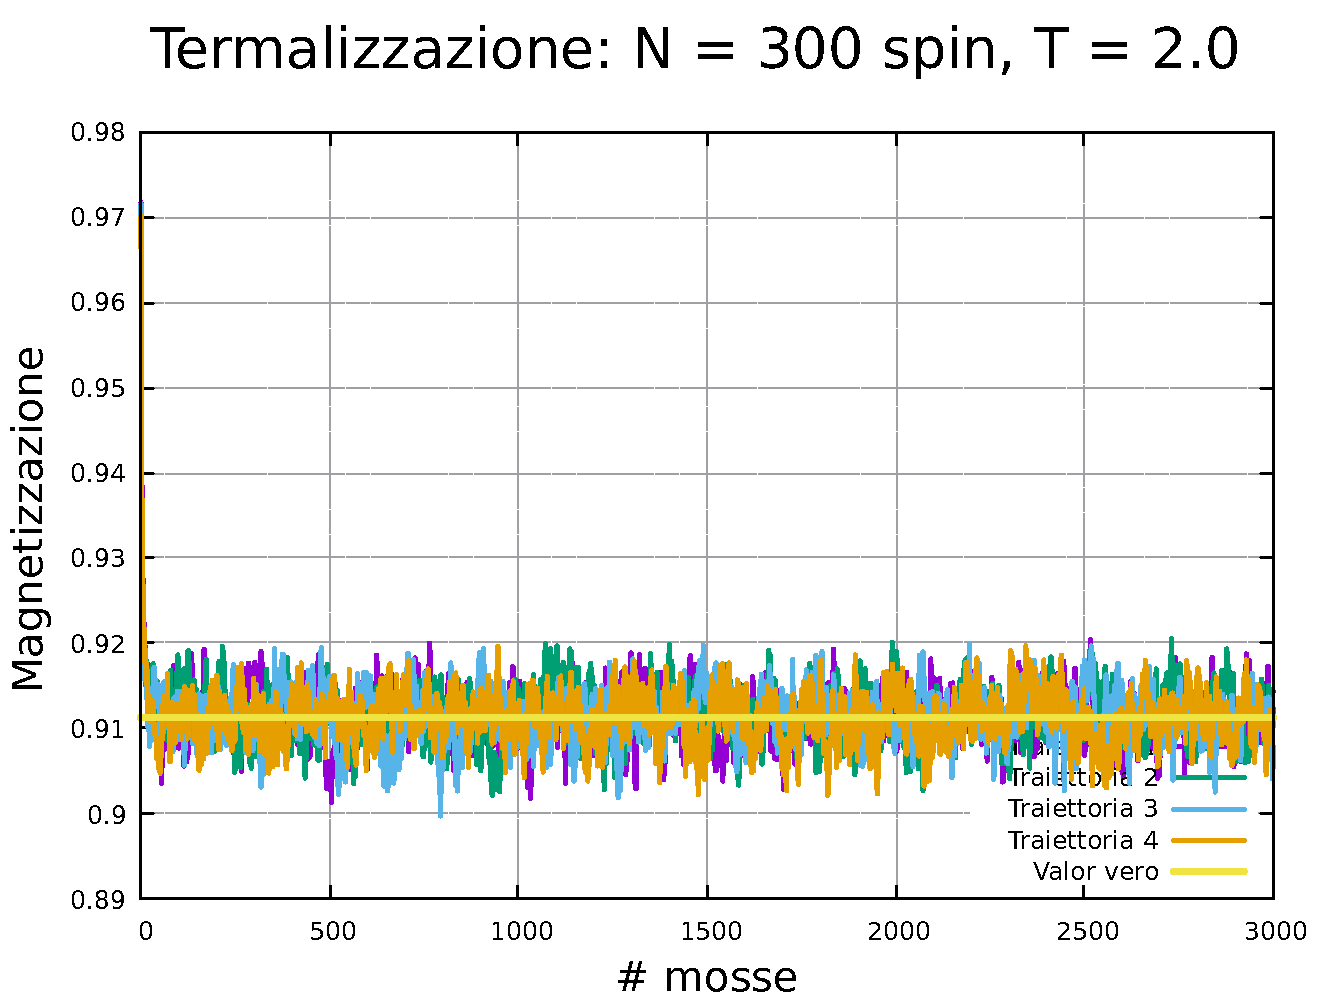
\includegraphics[page=1, width=\textwidth]{Immagini/simIsing2D/metro/term/term_300_2.0.pdf}
        \caption{$T\,=\,2.0$}
      \end{minipage}\hfill
      \begin{minipage}{0.45\textwidth}  
        \centering
        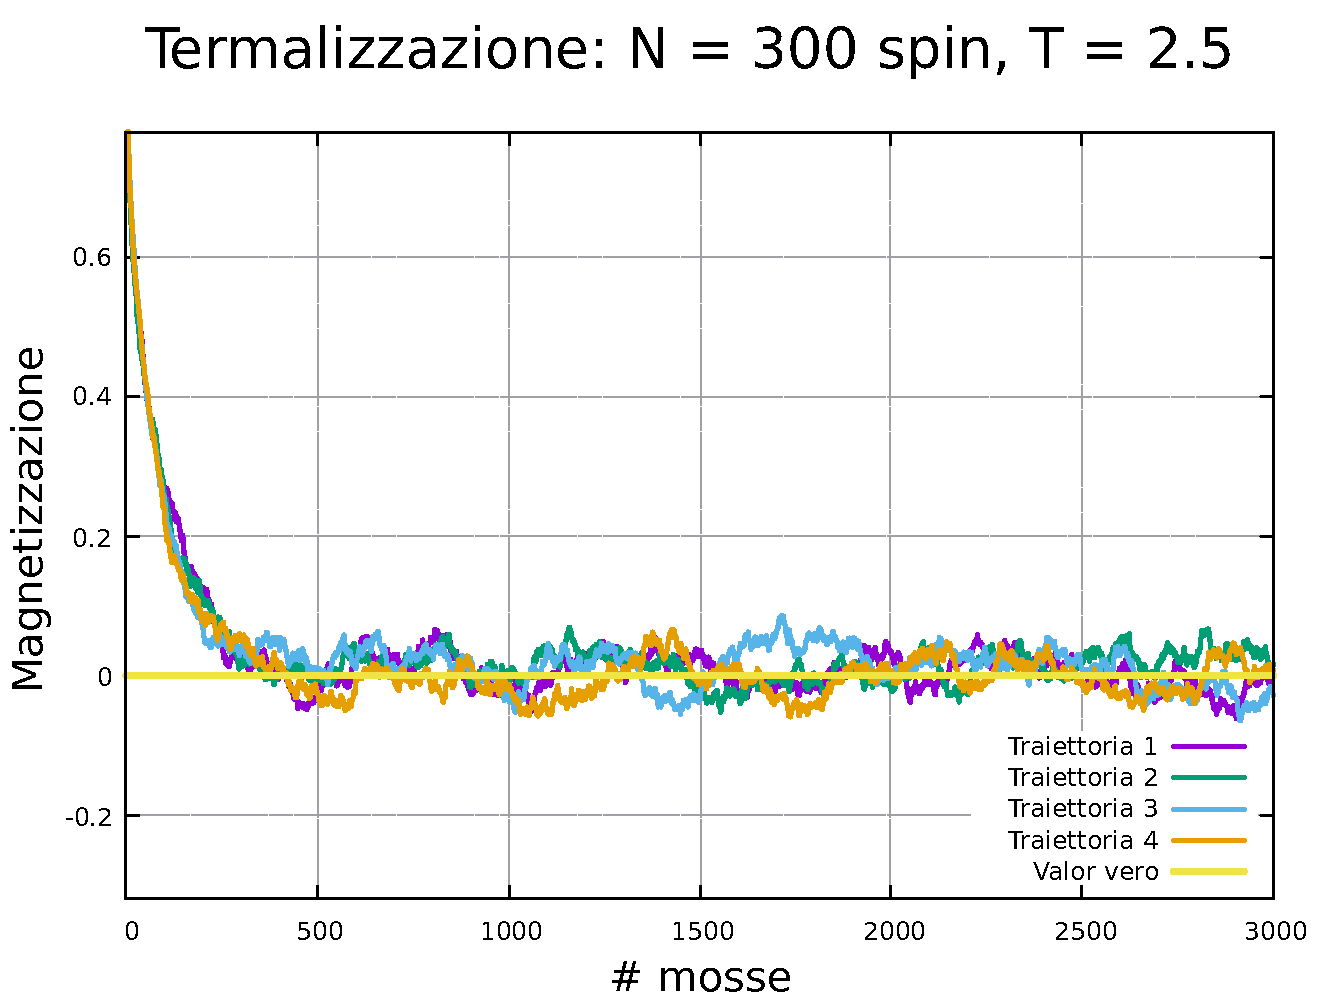
\includegraphics[page=1, width=\textwidth]{Immagini/simIsing2D/metro/term/term_300_2.5.pdf}
        \caption{$T\,=\,2.5$}
      \end{minipage}
    \vskip\baselineskip 
  
    \begin{minipage}{0.45\textwidth}  
      \centering
      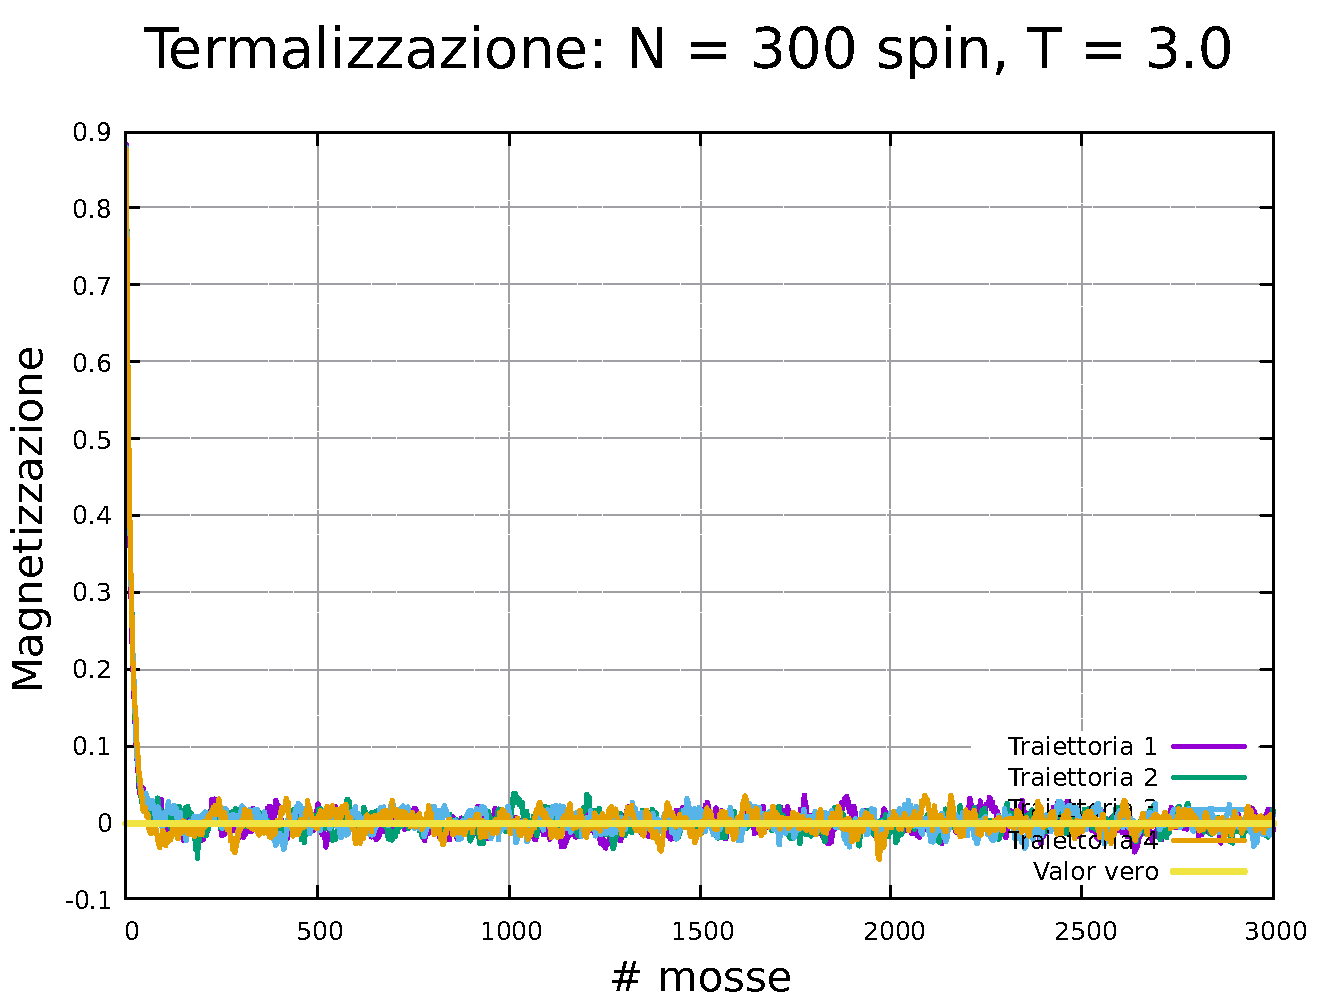
\includegraphics[page=1, width=\textwidth]{Immagini/simIsing2D/metro/term/term_300_3.0.pdf}
      \caption{$T\,=\,3.0$}
    \end{minipage}\hfill
    \begin{minipage}{0.45\textwidth}  
      \centering
      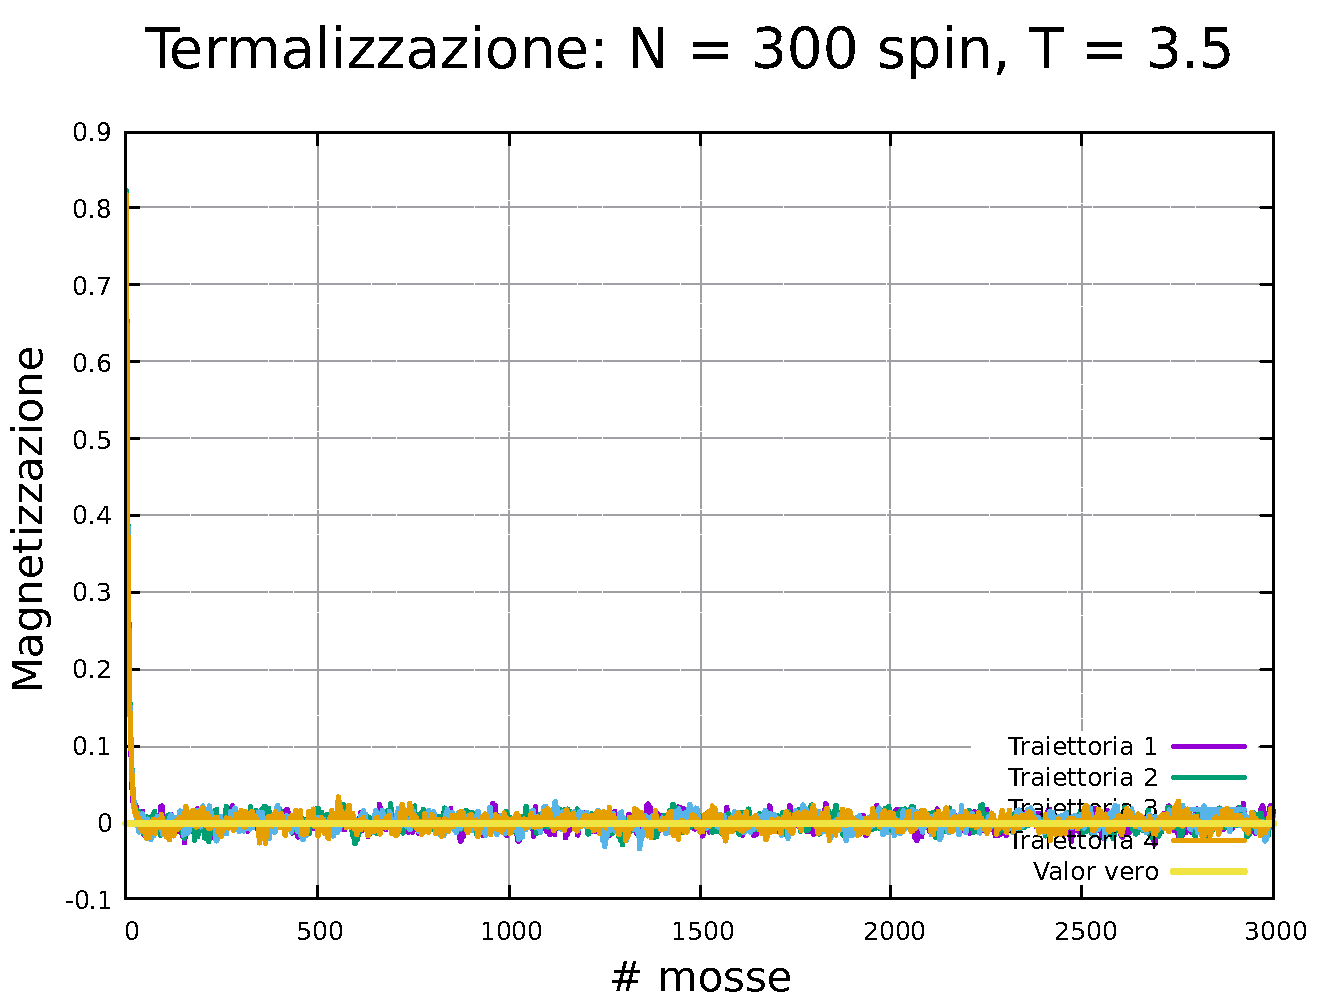
\includegraphics[page=1, width=\textwidth]{Immagini/simIsing2D/metro/term/term_300_3.5.pdf}
      \caption{$T\,=\,3.5$}
    \end{minipage}
    \caption{Studio della termalizzazione di un modello di Ising 2D costituito da $300 \times 300$ spin.}
\end{figure}

\vspace*{\fill}



\vspace*{\fill}

\begin{figure}[htbp]
    \centering
    \begin{minipage}{0.45\textwidth}  
      \centering
      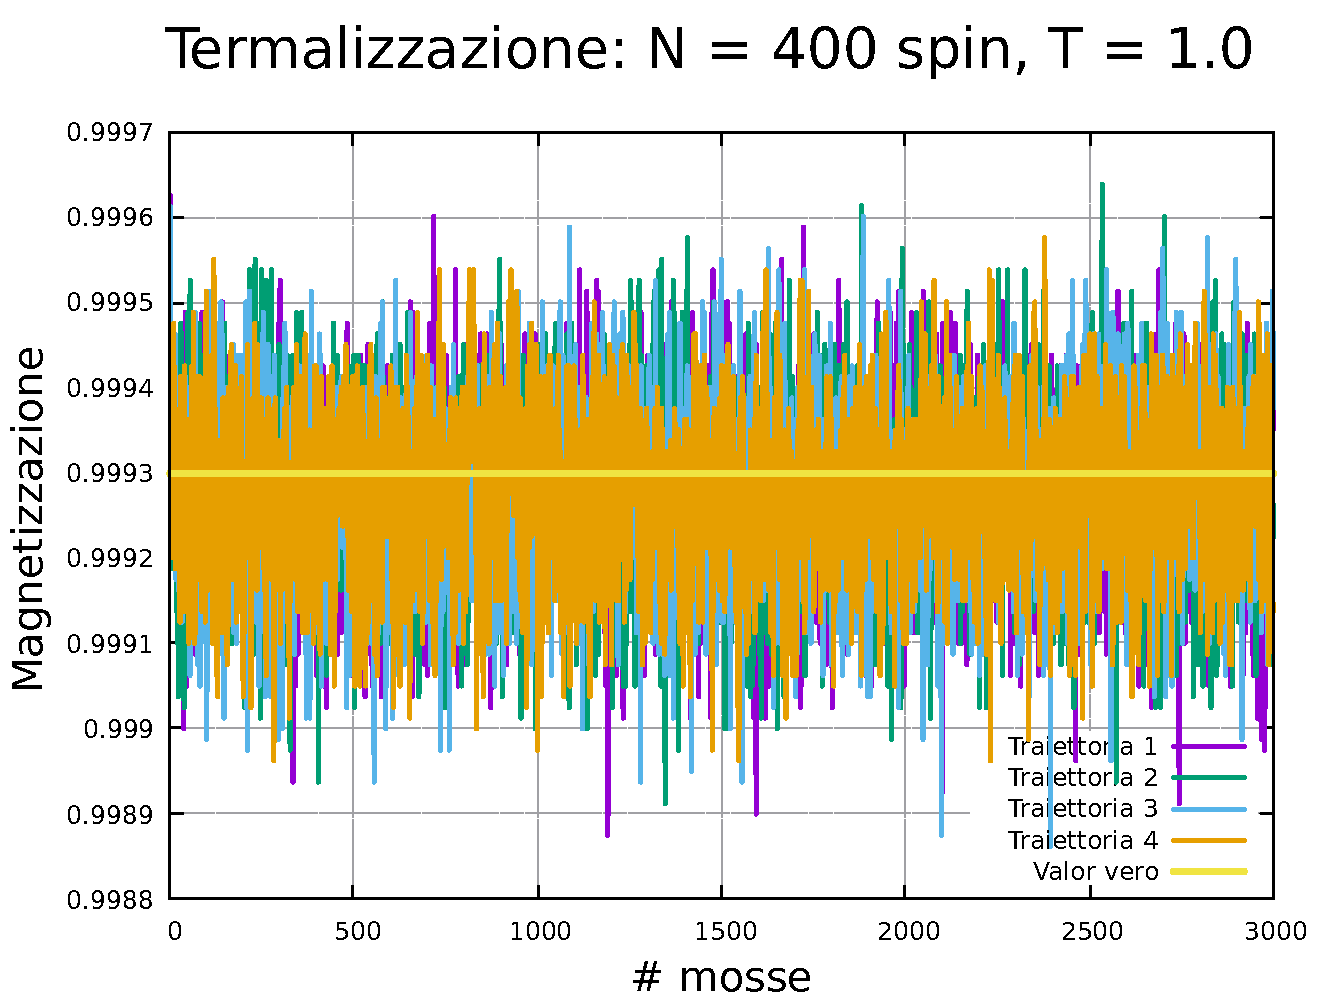
\includegraphics[page=1, width=\textwidth]{Immagini/simIsing2D/metro/term/term_400_1.0.pdf}
      \caption{$T\,=\,1.0$}
    \end{minipage}\hfill
    \begin{minipage}{0.45\textwidth}  
      \centering
      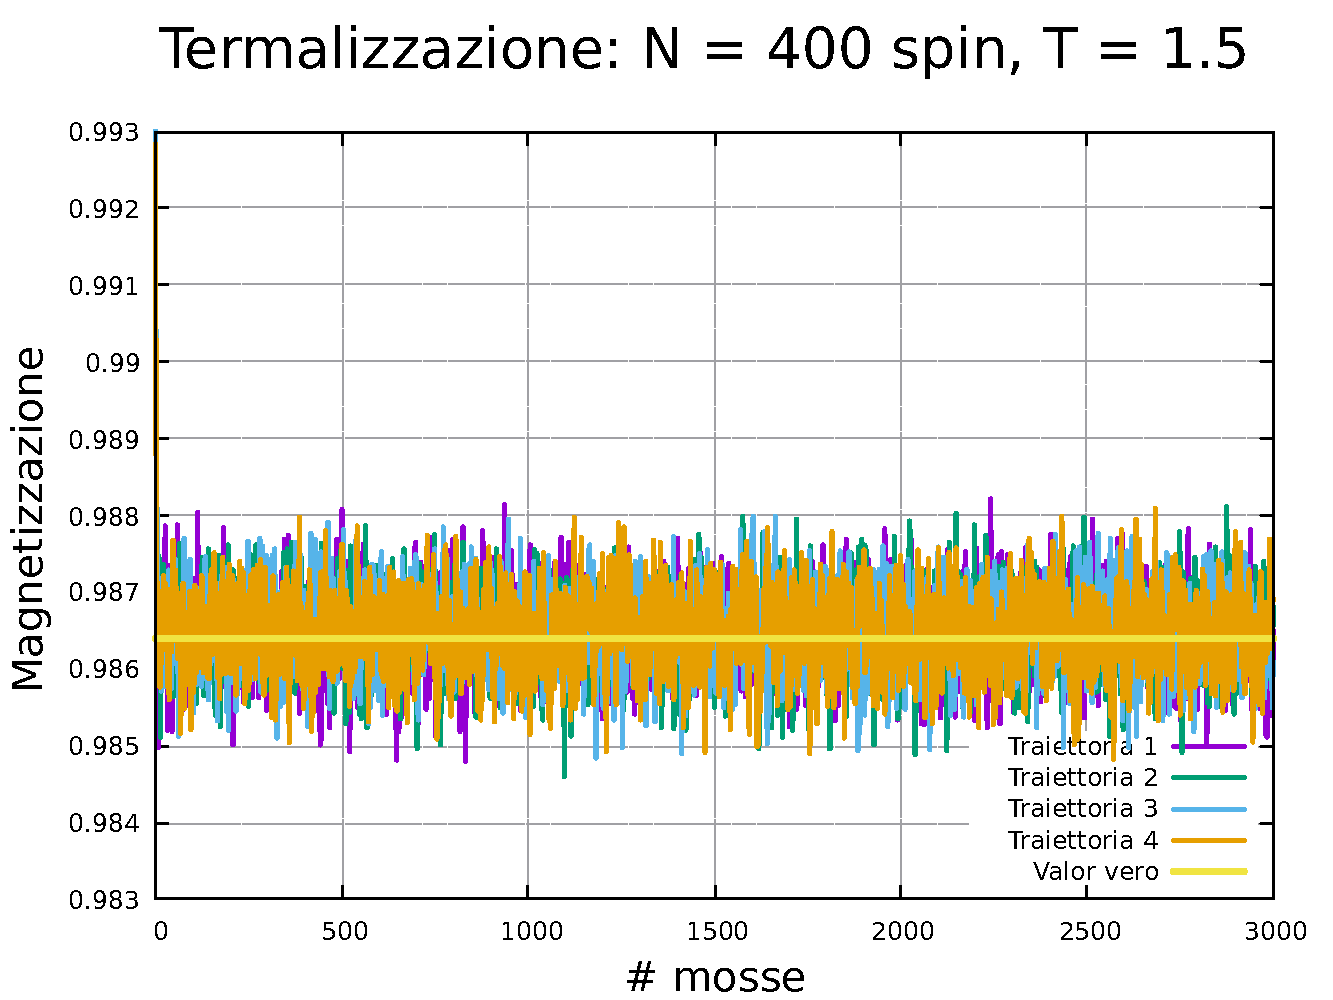
\includegraphics[page=1, width=\textwidth]{Immagini/simIsing2D/metro/term/term_400_1.5.pdf}
      \caption{$T\,=\,1.5$}
    \end{minipage}
    \vskip\baselineskip 

    \begin{minipage}{0.45\textwidth}  
        \centering
        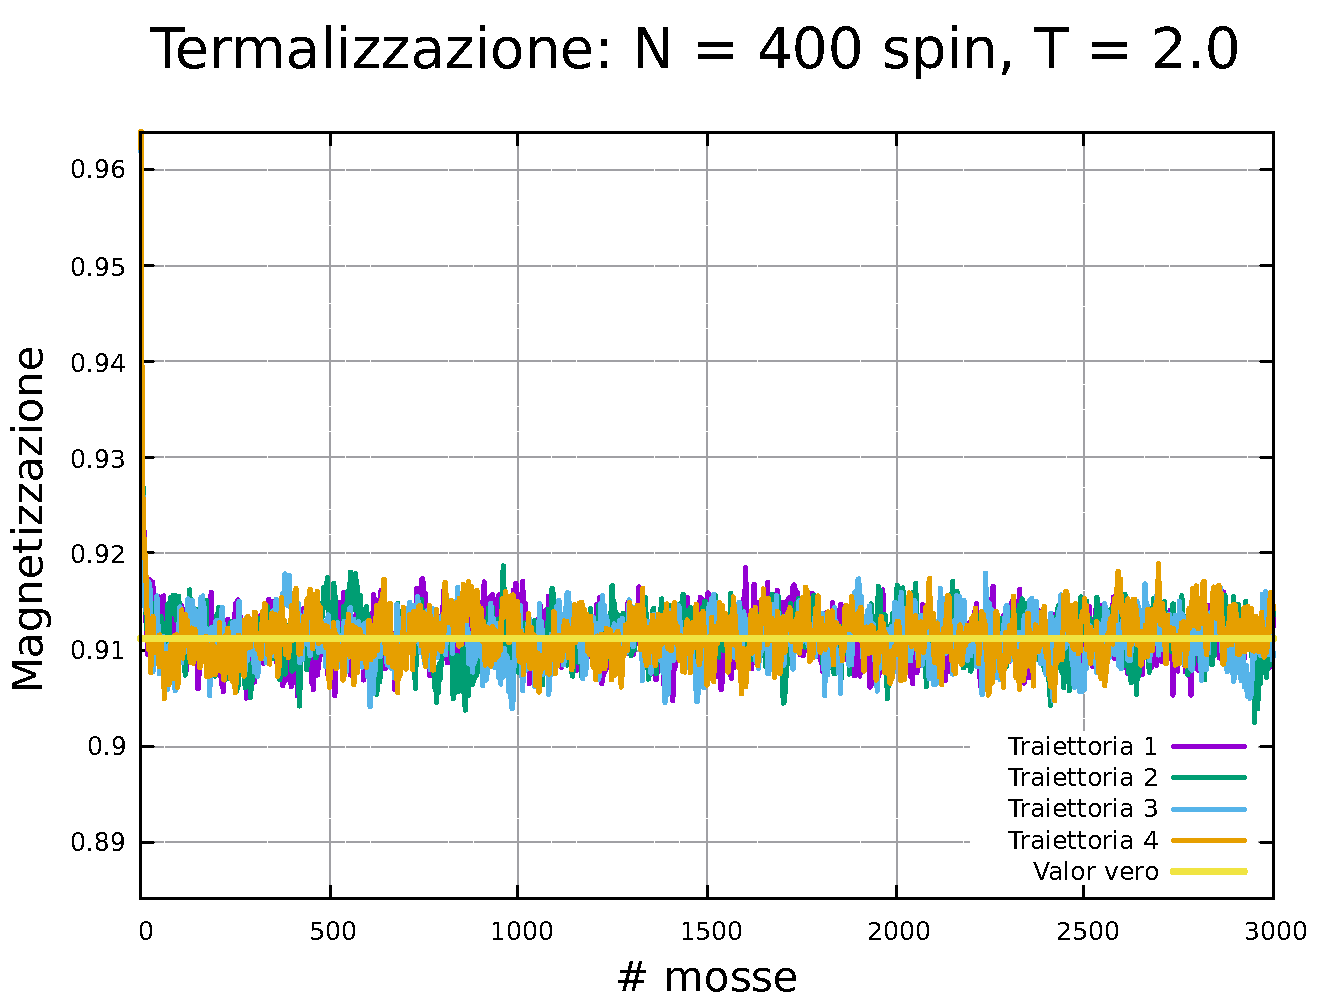
\includegraphics[page=1, width=\textwidth]{Immagini/simIsing2D/metro/term/term_400_2.0.pdf}
        \caption{$T\,=\,2.0$}
      \end{minipage}\hfill
      \begin{minipage}{0.45\textwidth}  
        \centering
        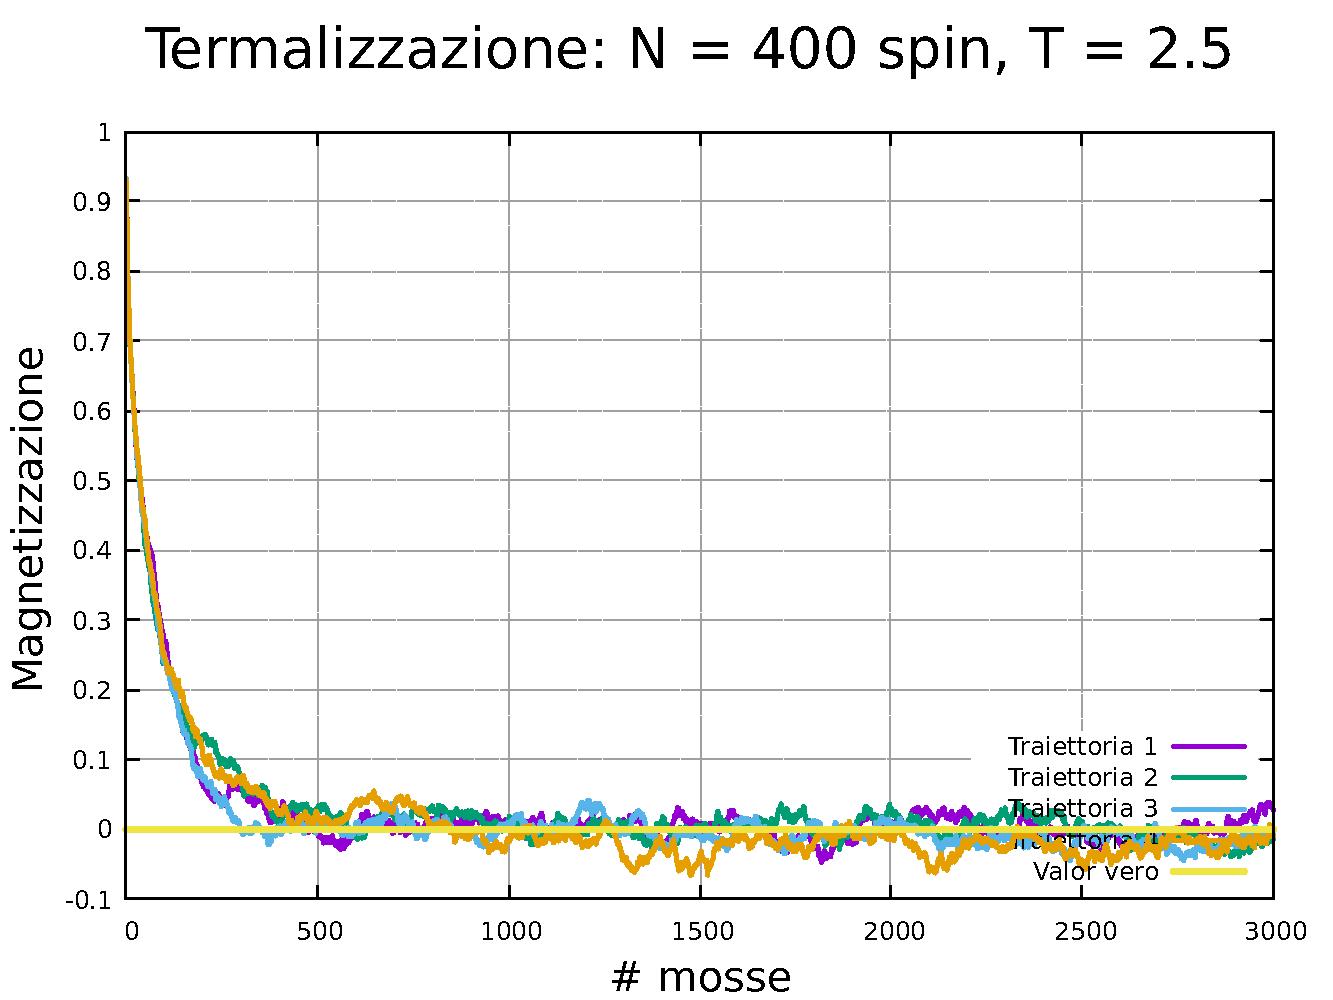
\includegraphics[page=1, width=\textwidth]{Immagini/simIsing2D/metro/term/term_400_2.5.pdf}
        \caption{$T\,=\,2.5$}
      \end{minipage}
    \vskip\baselineskip 
  
    \begin{minipage}{0.45\textwidth}  
      \centering
      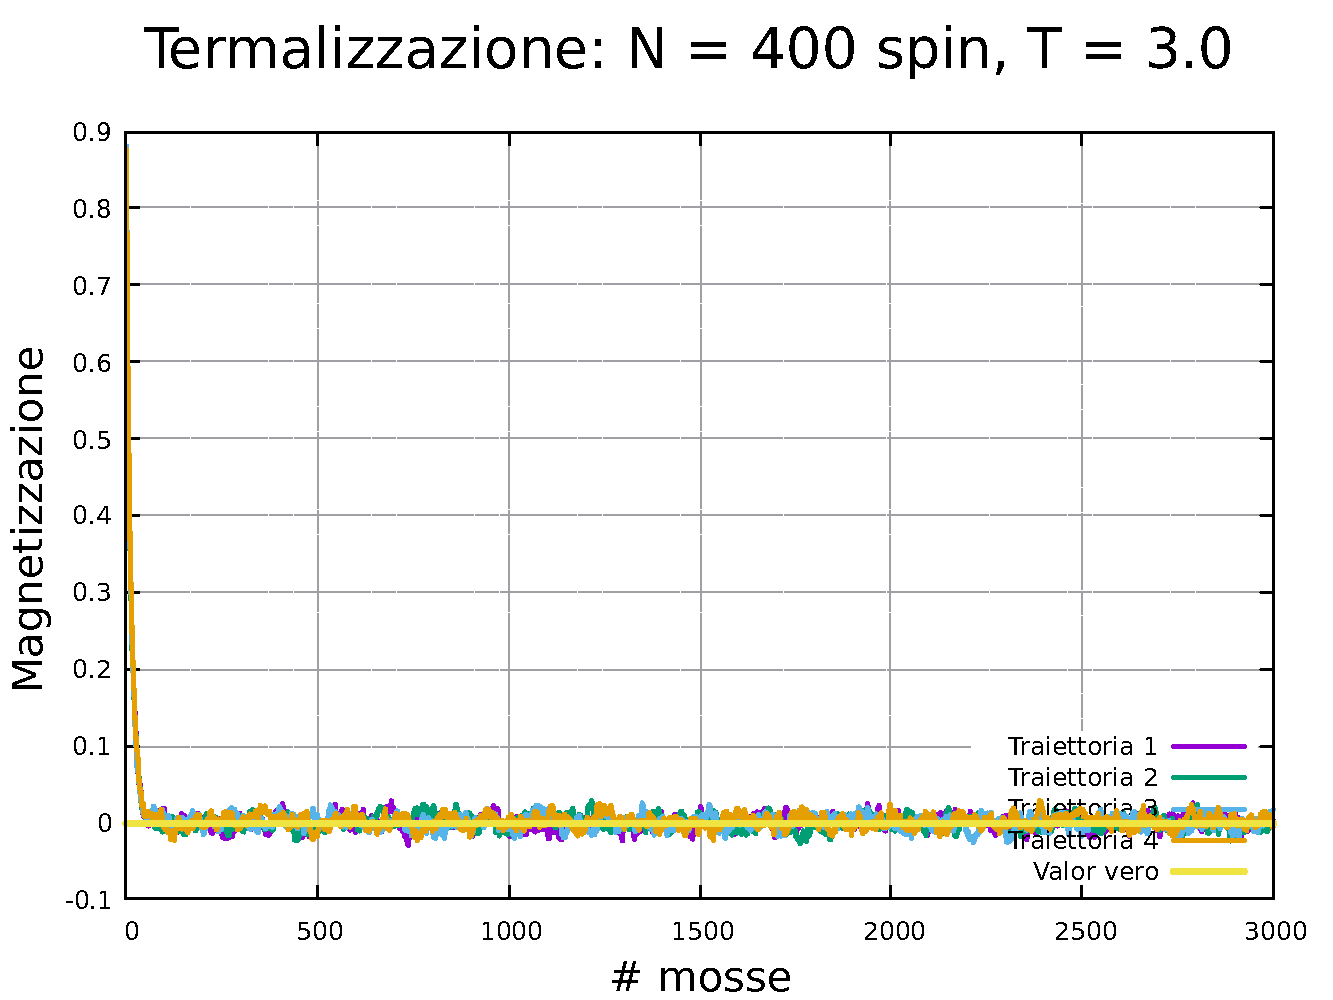
\includegraphics[page=1, width=\textwidth]{Immagini/simIsing2D/metro/term/term_400_3.0.pdf}
      \caption{$T\,=\,3.0$}
    \end{minipage}\hfill
    \begin{minipage}{0.45\textwidth}  
      \centering
      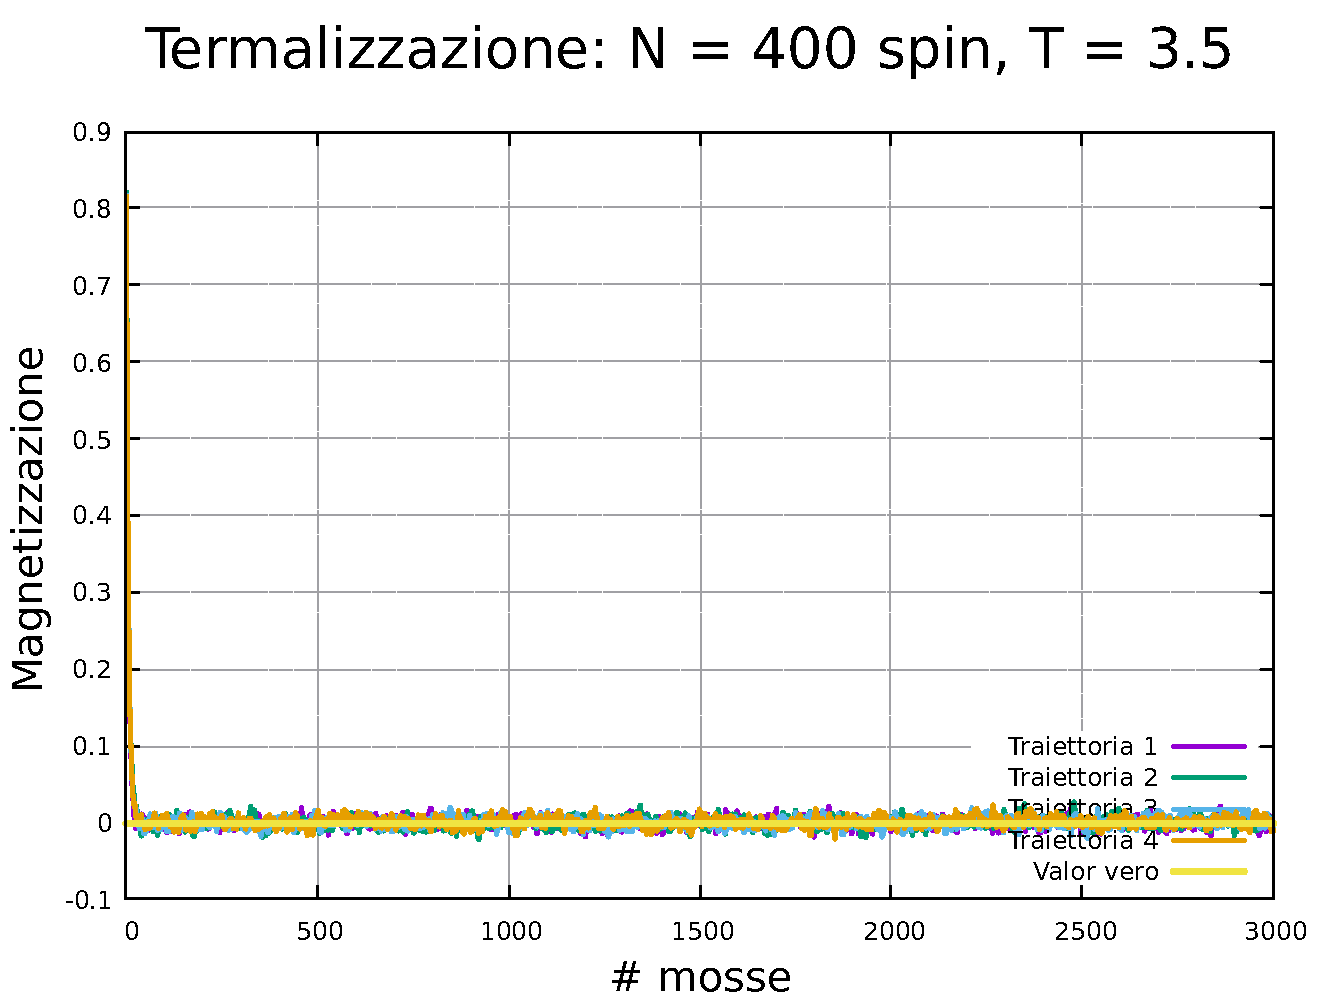
\includegraphics[page=1, width=\textwidth]{Immagini/simIsing2D/metro/term/term_400_3.5.pdf}
      \caption{$T\,=\,3.5$}
    \end{minipage}
    \caption{Studio della termalizzazione di un modello di Ising 2D costituito da $400 \times 400$ spin.}
\end{figure}

\vspace*{\fill}



\vspace*{\fill}

\begin{figure}[htbp]
    \centering
    \begin{minipage}{0.45\textwidth}  
      \centering
      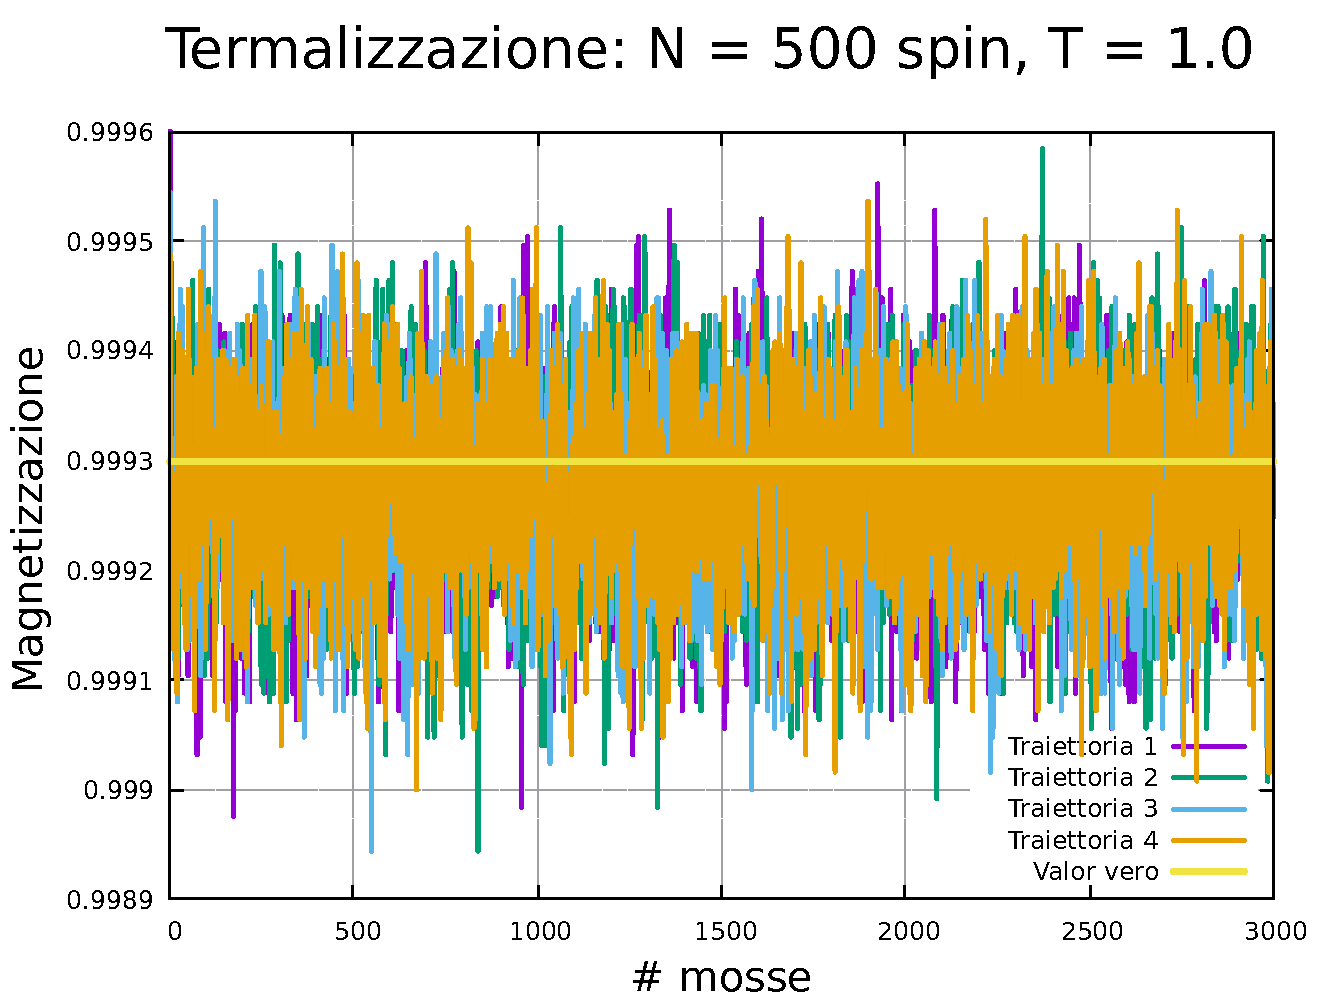
\includegraphics[page=1, width=\textwidth]{Immagini/simIsing2D/metro/term/term_500_1.0.pdf}
      \caption{$T\,=\,1.0$}
    \end{minipage}\hfill
    \begin{minipage}{0.45\textwidth}  
      \centering
      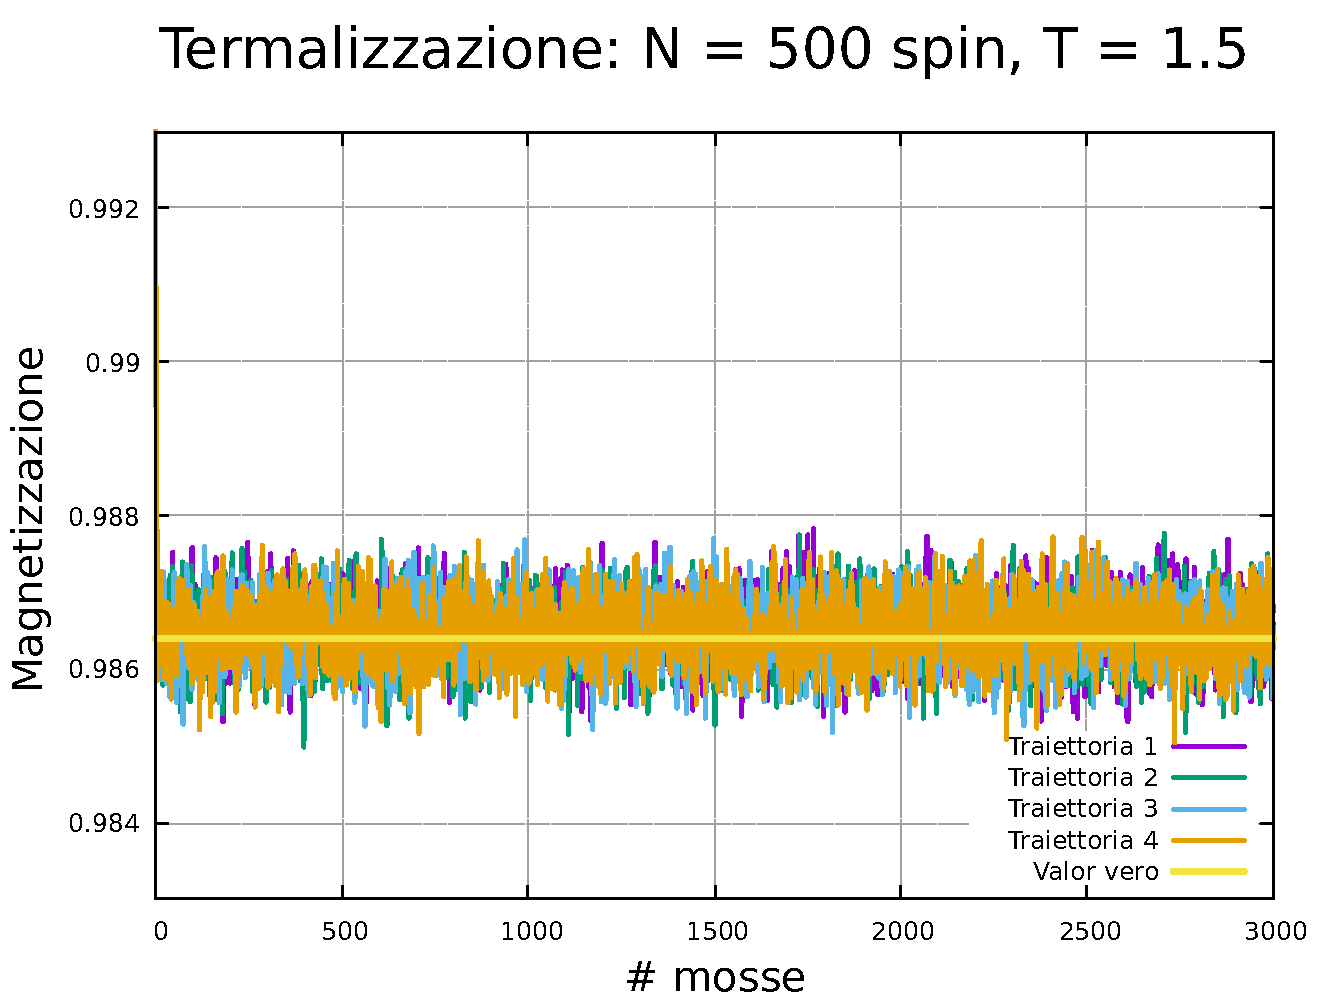
\includegraphics[page=1, width=\textwidth]{Immagini/simIsing2D/metro/term/term_500_1.5.pdf}
      \caption{$T\,=\,1.5$}
    \end{minipage}
    \vskip\baselineskip 

    \begin{minipage}{0.45\textwidth}  
        \centering
        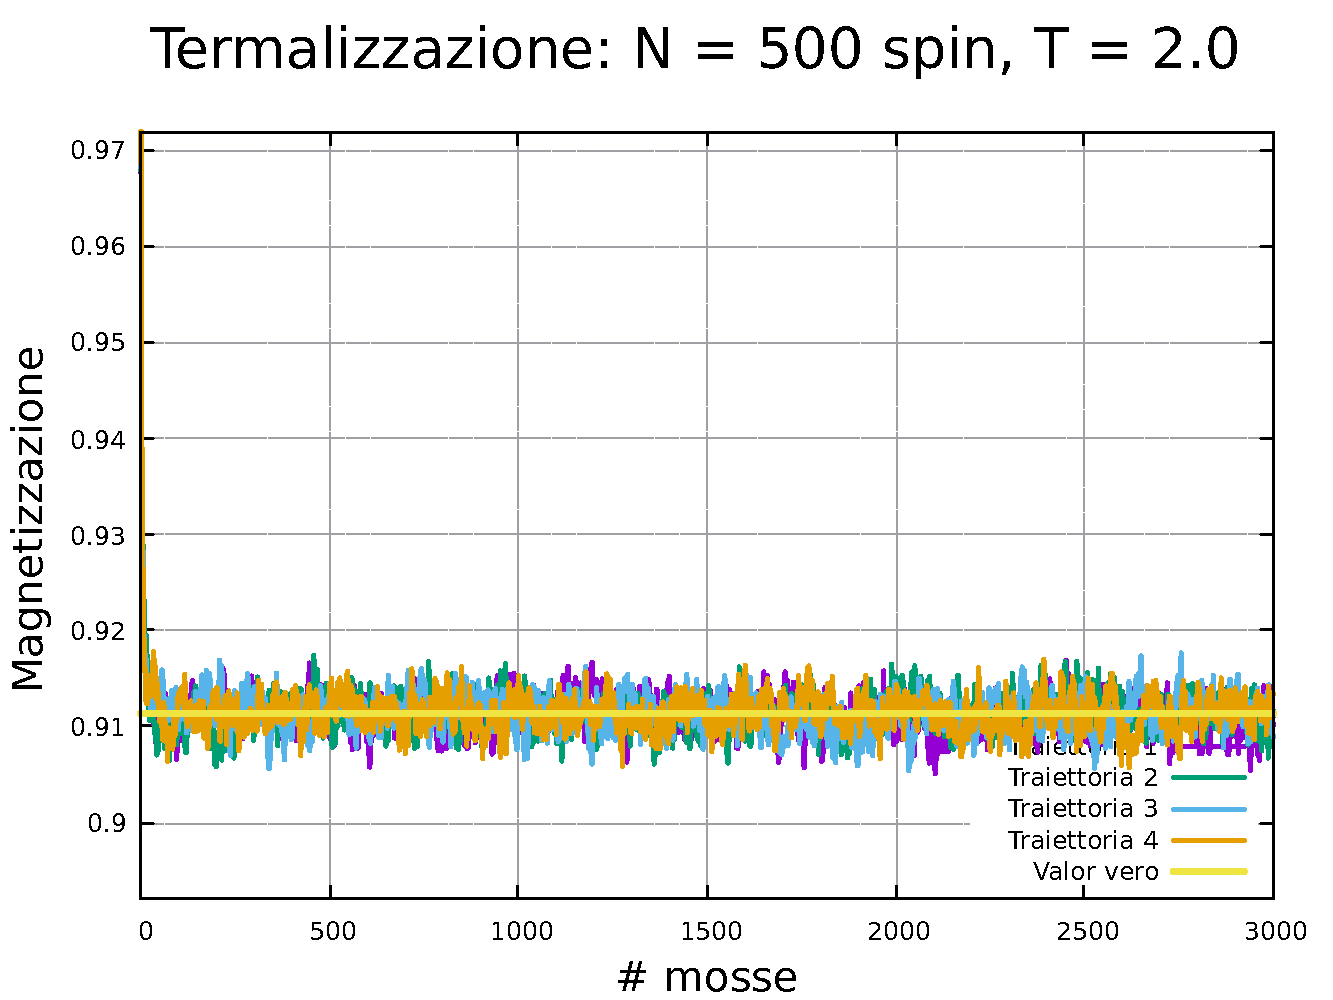
\includegraphics[page=1, width=\textwidth]{Immagini/simIsing2D/metro/term/term_500_2.0.pdf}
        \caption{$T\,=\,2.0$}
      \end{minipage}\hfill
      \begin{minipage}{0.45\textwidth}  
        \centering
        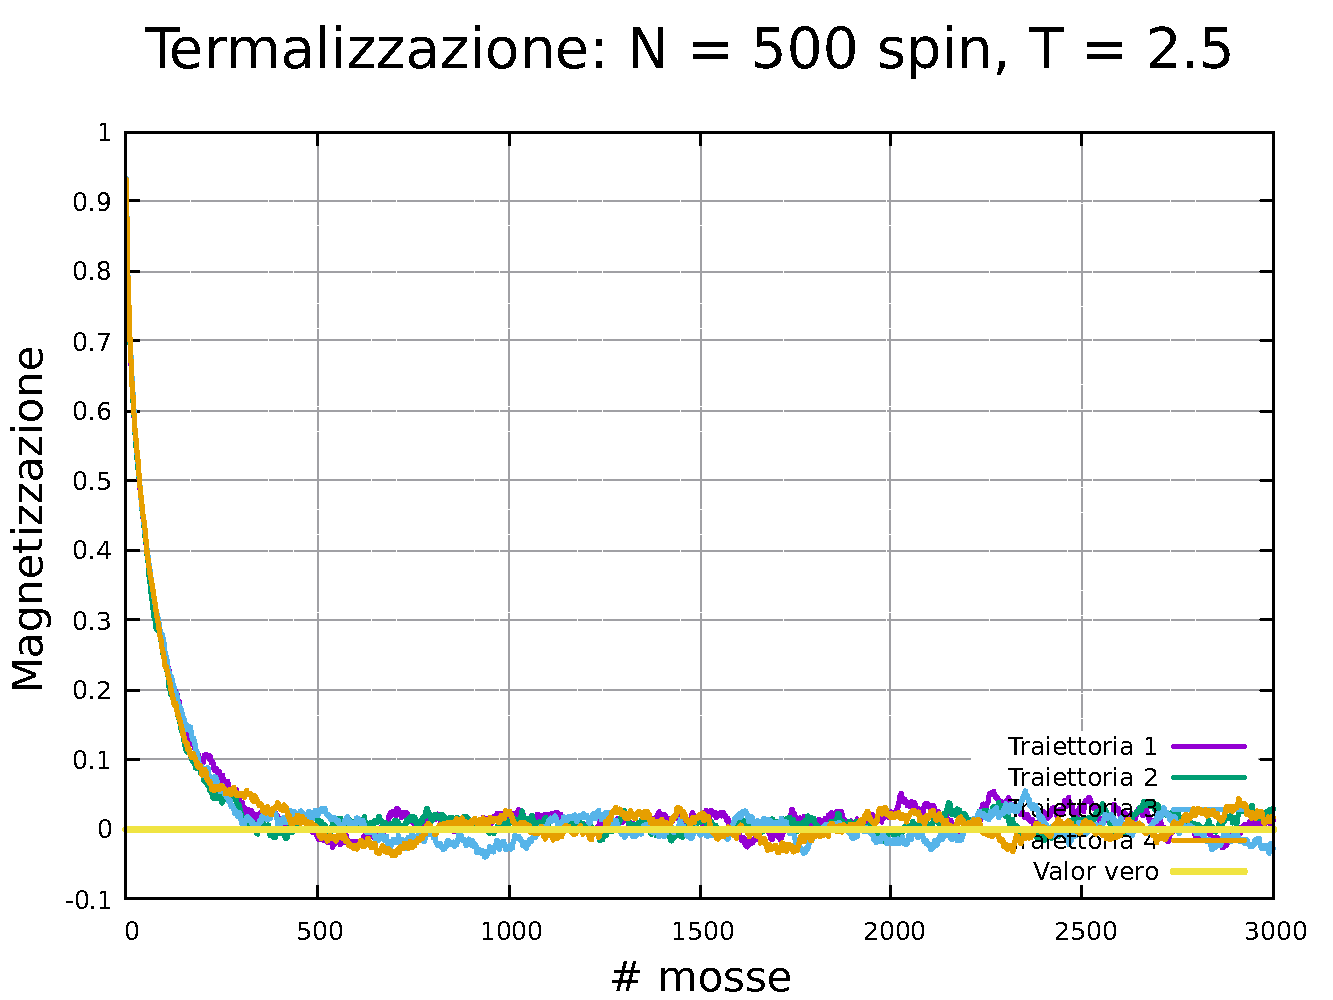
\includegraphics[page=1, width=\textwidth]{Immagini/simIsing2D/metro/term/term_500_2.5.pdf}
        \caption{$T\,=\,2.5$}
      \end{minipage}
    \vskip\baselineskip 
  
    \begin{minipage}{0.45\textwidth}  
      \centering
      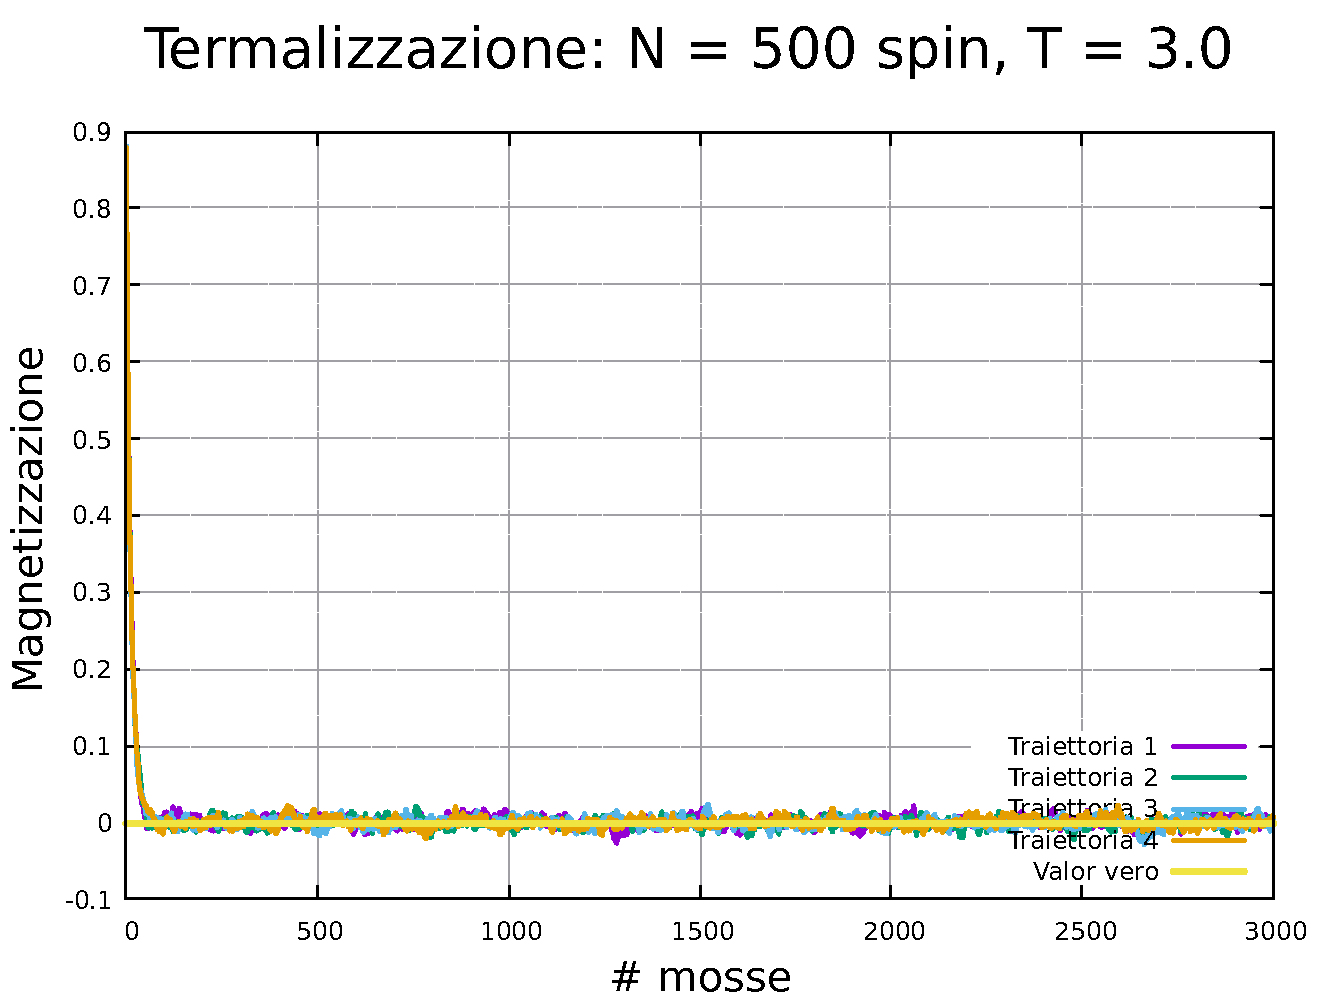
\includegraphics[page=1, width=\textwidth]{Immagini/simIsing2D/metro/term/term_500_3.0.pdf}
      \caption{$T\,=\,3.0$}
    \end{minipage}\hfill
    \begin{minipage}{0.45\textwidth}  
      \centering
      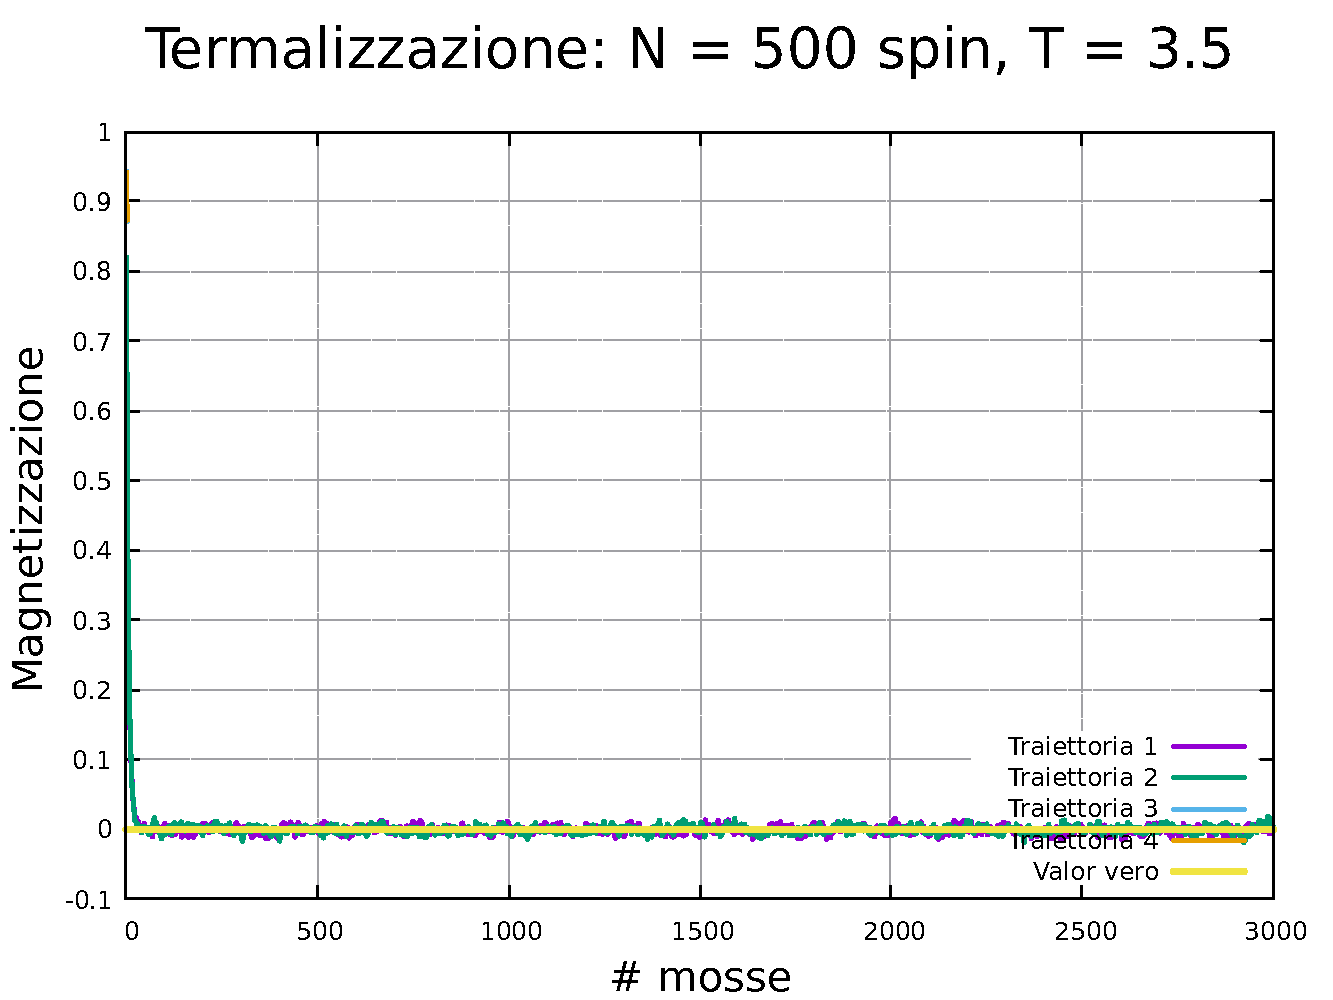
\includegraphics[page=1, width=\textwidth]{Immagini/simIsing2D/metro/term/term_500_3.5.pdf}
      \caption{$T\,=\,3.5$}
    \end{minipage}
    \caption{Studio della termalizzazione di un modello di Ising 2D costituito da $500 \times 500$ spin.}
\end{figure}

\vspace*{\fill}
